%%%%%%%%%%%%%%%%%%%%%%% file template.tex %%%%%%%%%%%%%%%%%%%%%%%%%
%
% This is a general template file for the LaTeX package SVJour3
% for Springer journals.          Springer Heidelberg 2010/09/16
%
% Copy it to a new file with a new name and use it as the basis
% for your article. Delete % signs as needed.
%
% This template includes a few options for different layouts and
% content for various journals. Please consult a previous issue of
% your journal as needed.
%
%%%%%%%%%%%%%%%%%%%%%%%%%%%%%%%%%%%%%%%%%%%%%%%%%%%%%%%%%%%%%%%%%%%
%
% First comes an example EPS file -- just ignore it and
% proceed on the \documentclass line
% your LaTeX will extract the file if required
%\documentclass{svjour3}                     % onecolumn (standard format)
%\documentclass[smallcondensed]{svjour3}     % onecolumn (ditto)
\documentclass[smallextended]{svjour3}       % onecolumn (second format)
%\documentclass[twocolumn]{svjour3}          % twocolumn
%
\smartqed  % flush right qed marks, e.g. at end of proof
%
\usepackage[utf8]{inputenc}
\usepackage[T1]{fontenc}
\usepackage{amsmath,amssymb,amsfonts}
\usepackage{algorithmic}
\usepackage{graphicx}
\usepackage{textcomp}
\usepackage{booktabs}
\usepackage{framed}
\usepackage{float}
\usepackage{xcolor}
\usepackage{footnote}
\usepackage{xfrac}
\usepackage{balance}
\usepackage{hyperref}
\usepackage{array}
\usepackage{subfigure}
\usepackage{changepage}
\usepackage{listings}

\newcolumntype{L}[1]{>{\raggedright\let\newline\\\arraybackslash\hspace{0pt}}m{#1}}

\definecolor{mygreen}{rgb}{0,0.6,0}
\definecolor{lightgreen}{rgb}{0.6,0.9,0.6}
\definecolor{lightyellow}{rgb}{0.9,0.9,0.6}
\definecolor{lightorange}{rgb}{0.9,0.8,0.6}
\definecolor{lightred}{rgb}{0.9,0.7,0.7}
\definecolor{mygray}{rgb}{0.5,0.5,0.5}
\definecolor{lightgray}{rgb}{0.8,0.8,0.8}
\definecolor{mymauve}{rgb}{0.58,0,0.82}

\usepackage{pifont}
\newcommand{\lstbg}[3][0pt]{{\fboxsep#1\colorbox{#2}{\strut #3}}}

\lstdefinestyle{CStyle} {
    language=C,
    backgroundcolor=\color{white},   % choose the background color
    basicstyle=\ttfamily\scriptsize,        % size of fonts used for the code
    breaklines=true,                 % automatic line breaking only at whitespace
    captionpos=b,                    % sets the caption-position to bottom
    commentstyle=\color{mygray}\bfseries,    % comment style
    escapeinside={\%*}{*)},          % if you want to add LaTeX within your code
    keywordstyle=\color{blue},       % keyword style
    stringstyle=\color{mymauve},     % string literal style
    frame=single,
    numbers=left,
    stepnumber=1,
    xleftmargin=2em,
    escapeinside={/*!}{!*/},
    moredelim=**[l][\color{mygreen}]{+\ },
    moredelim=*[l][\color{red}]{-\ }
}

\lstdefinestyle{JavaStyle} {
    language=Java,
    backgroundcolor=\color{white},   % choose the background color
    basicstyle=\ttfamily\scriptsize,        % size of fonts used for the code
    breaklines=true,                 % automatic line breaking only at whitespace
    captionpos=b,                    % sets the caption-position to bottom
    commentstyle=\color{mygray}\bfseries,    % comment style
    escapeinside={\%*}{*)},          % if you want to add LaTeX within your code
    keywordstyle=\color{blue},       % keyword style
    stringstyle=\color{mymauve},     % string literal style
    frame=single,
    numbers=left,
    stepnumber=1,
    xleftmargin=2em,
    escapeinside={/*!}{!*/},
    moredelim=**[l][\color{mygreen}]{+\ },
    moredelim=*[l][\color{red}]{-\ }
}

\lstdefinestyle{PHPStyle} {
    language=PHP,
    alsolanguage=HTML,
    backgroundcolor=\color{white},   % choose the background color
    basicstyle=\ttfamily\scriptsize,        % size of fonts used for the code
    breaklines=true,                 % automatic line breaking only at whitespace
    captionpos=b,                    % sets the caption-position to bottom
    commentstyle=\color{mygray}\bfseries,    % comment style
    escapeinside={\%*}{*)},          % if you want to add LaTeX within your code
    keywordstyle=\color{blue},       % keyword style
    stringstyle=\color{mymauve},     % string literal style
    frame=single,
	numbers=left,
    stepnumber=1,
	xleftmargin=2em,
    escapeinside={/*!}{!*/},
    moredelim=**[l][\color{mygreen}]{+\ },
    moredelim=*[l][\color{red}]{-\ }
}

\newcounter{lstannotation}
\setcounter{lstannotation}{0}
\renewcommand{\thelstannotation}{\ding{\number\numexpr181+\arabic{lstannotation}}}
\newcommand{\annotation}[1]{\refstepcounter{lstannotation}\label{#1}\thelstannotation}

\newboolean{showcomments}
\setboolean{showcomments}{true}
%\setboolean{showcomments}{false}

\ifthenelse{\boolean{showcomments}}
  {\newcommand{\nb}[3]{
  {\color{#2}\small\fbox{\bfseries\sffamily\scriptsize#1}}
  {\color{#2}\sffamily\small$\triangleright~$\textit{\small #3}$~\triangleleft$}
  }
  }
  {\newcommand{\nb}[3]{}
  }

\newcommand\Sofia[1]{\nb{Sofia}{red}{#1}}
\newcommand\Luis[1]{\nb{Luis}{mygreen}{#1}}
\newcommand\Rui[1]{\nb{Rui}{blue}{#1}}

\makeatletter
\newcommand\footnoteref[1]{\protected@xdef\@thefnmark{\ref{#1}}\@footnotemark}
\makeatother

%
% \usepackage{mathptmx}      % use Times fonts if available on your TeX system
%
% insert here the call for the packages your document requires
%\usepackage{latexsym}
% etc.
%
% please place your own definitions here and don't use \def but
% \newcommand{}{}
%
% Insert the name of "your journal" with
% \journalname{myjournal}
%
\begin{document}

\title{Fixing Vulnerabilities Potentially Hinders Maintainability}

\author{Sofia Reis         \and
        Rui Abreu           \and
        Luis Cruz
}

\institute{Sofia Reis \at
			INESC ID and IST, University of Lisbon, Lisbon, Portugal\\
            \email{sofia.o.reis@tecnico.ulisboa.pt}   
			\and
			Rui Abreu \at
			INESC ID and FEUP, University of Porto, Porto, Portugal\\
			\email{rui@computer.org}
           \and
			Luis Cruz \at
			Delft University of Technology, Delft, The Netherlands\\
			\email{L.Cruz@tudelft.nl}
}

\date{Received: date / Accepted: date}


\maketitle

\begin{abstract}
Security is a requirement of utmost importance to produce 
high-quality software. However, there is still a considerable amount 
of vulnerabilities being discovered and fixed, almost weekly. We 
hypothesize that developers affect the maintainability of their 
codebases when patching vulnerabilities. This paper evaluates the 
impact of patches to improve security on the maintainability of 
open-source software. Maintainability is measured based on the 
Better Code Hub’s model of 10 guidelines on a dataset including 
1300 security-related commits. Results show evidence of a trade-off 
between security and maintainability in $41.9\%$ of the cases, i.e., developers 
may hinder software maintainability. More than $35\%$ of security 
patches increased software complexity and the percentage 
of LOCs per unit. The implications of our study 
are that changes to codebases while patching vulnerabilities need to 
be performed with extra care; tools for patch risk assessment should 
be integrate into the CI/CD pipeline; computer science curricula 
needs to be updated; and, more secure programming languages are 
necessary.
\keywords{Software Security \and Software Maintenance \and Open-Source Software}
\end{abstract}


\section{Introduction}
%
Software quality is important because it is ultimately related to 
the overall cost of developing and maintaining software 
applications, security and safety~\cite{slaughter1998evaluating}. Software quality 
characteristics include, but are not limited to functional 
correctness, reliability, usability, maintainability, evolvavility 
and security. Security is an essential non-functional requirement 
during the development of software systems. In $2011$, the 
International Organization for Standardization (ISO) issued an 
update for software product quality ISO/IEC 25010 considering 
\emph{Security} as one of the main software product quality 
characteristics~\cite{iso:2011}. However, there is still 
a considerable amount of vulnerabilities being discovered and fixed, 
almost weekly, as disclosed by the Zero Day Initiative 
website\footnote{Zero Day Initiative website available at 
\url{https://www.zerodayinitiative.com/advisories/published/} 
(Accessed on \today{})}. 

Researchers found a correlation between the presence of 
vulnerabilities on software and code complexity~\cite{shin2010evaluating,10.1145/1774088.1774504}. 
Security experts claim that complexity hides bugs that may result in 
security vulnerabilities~\cite{mcgraw2004software,schneier2006beyond}. In 
practice, an attacker only needs to find one way into the system 
while a defender needs to find and mitigate all the security issues. 
Complex code is difficult to understand, maintain and 
test~\cite{1702388}. Thus, the task of a developer gets harder as the 
codebase grows in size and complexity. But the risk can be minimized 
by writing clean and maintainable code. 

ISO describes \textit{software maintainability} as ``the degree of 
effectiveness and efficiency with which a software product or system 
can be modified to improve it, correct it or adapt it to changes in 
environment, and in requirements'' on software quality ISO/IEC 
25010~\cite{iso:2011}. Thereby, maintainable security may be 
defined, briefly, as the degree of effectiveness and efficiency with 
which software can be changed to mitigate a security 
vulnerability---corrective maintenance.
% (hopefully, without introducing new ones). 
However, many developers still lack knowledge on the best 
practices to deliver and maintain secure and high-quality 
software~\cite{Pothamsetty:2005:SEL:1107622.1107635,8077802}. In a 
world where zero-day vulnerabilities are constantly emerging, 
mitigation needs to be fast and efficient. Therefore, it 
is important to write maintainable code to support the production of 
more secure software---maintainable code is less complex and, 
consequently, less prone to
vulnerabilities~\cite{shin2010evaluating,10.1145/1774088.1774504}---
and, prevent the introduction of new vulnerabilities. 

% Unmaintainable code is hard to test, analyze and re-use. Therefore,
% it is important to write maintainable code to support the production
% of more secure software and prevent
% the introduction of new vulnerabilities in the code bases.
%
Static analysis tools (SATs) have been built to automatically detect software 
vulnerabilities (e.g., FindBugs, Infer and more). Developers
use those tools to locate the issues in the code. However,
while performing the patches to those issues, SATs are not 
capable of providing information on the quality of the patch.
Improving software security is not a trivial task and 
requires implementing patches that might affect software 
maintainability. Our hypothesis is that some of these patches may 
have a negative impact on the software maintainability and, 
possibly, even be the cause of the introduction of new 
vulnerabilities---harming software reliability and introducing 
technical debt. Research found that $34\%$ of the security patches 
performed introduce new problems and $52\%$ are incomplete and do not 
fully secure systems~\cite{10.1145/3133956.3134072}. Therefore, in this paper, 
we present an empirical study on the impact of patches of 
vulnerabilities on software maintenance across open-source software.
We arguee that tools that assess these type of metrics may
complement SATs with valuable information to help the developer
understand better the risk of its patch.

As ISO does not provide any specific guidelines/formulas to 
calculate maintainability, we resort to Software Improvement Group 
(SIG\footnote{SIG's website: 
\url{https://www.sig.eu/} (Accessed on \today{})})'s web-based source 
code analysis service Better Code Hub (BCH)\footnote{BCH's 
website: \url{https://bettercodehub.com/} (Accessed on \today{})}  
to compute the software compliance with a set of $10$ 
guidelines/metrics to produce quality software based in ISO/IEC 
$25010$~\cite{Visser:2016:OREILLY}. SIG 
has been helping business and technology leaders drive their organizational 
objectives by fundamentally improving the health and security of 
their software applications for more than 20 years. Their 
models are scientifically proven and certified~\cite{4335232,5609747,6113040,baggen2012}.

There are other well-known 
standards and models that have been proposed to increase software 
security: Common Criteria~\cite{common:2009} which received
negative criticism regarding the costs associated and poor technical 
evaluation; the OWASP Application Security Verification 
Standard (ASVS)~\cite{oswap:2009} which is focused only on web 
applications, and a model proposed by Xu et al. ($2013$)
~\cite{6616351} for rating software security (arguably, it was one 
of the first steps taken by SIG to introduce security on their 
maintainability model). Nevertheless, our study uses BCH to provide 
an assessment of maintainability in software for the following 
reasons: BCH integrates a total of $10$ different code metrics; and, 
code metrics were empirically validated in previous 
work~\cite{Bijlsma:2012:FIR:2317098.2317124,8530041,8919169,8785997}.

From a methodological perspective, we leveraged a dataset of $1300$ 
security patches collected from open-source software. We calculate 
software maintainability before and after the patch to measure its 
impact. This empirical study presents evidence that changes applied 
in the codebases to patch vulnerabilities affect code 
maintainability. Results also suggest that developers 
should pay different levels of attention to different severity 
levels and classes of weaknesses when patching vulnerabilities. We 
also show that patches in programming languages such as, 
\emph{C/C++}, \emph{Ruby} and \emph{PHP}, may have a more negative 
impact in software maintainability. Little information is known 
about the impact of security patches on software 
maintainability. Developers need to be aware of the impact of their 
changes on software maintainability while patching security 
vulnerabilities. The harm of maintainability can increase the time 
of response of future mitigations or even other maintainability 
tasks. Thus, it is of utmost importance to find means to assist 
mitigation and reduce its risks. With this study, we intend to 
highlight the need for tools to assess the impact of patches on 
software maintainability~\cite{4724577}; the importance of 
integrating maintainable security in computer science curricula; 
and, the demand for better programming languages, designed by 
leveraging security principles~\cite{kurilova2014wyvern,10.1145/2489828.2489830}. 
 
This research performs the following main contributions:
%
\begin{itemize}
	\vspace{-0.3em}
  \item Evidence that supports the trade-off between security and 
  maintainability: developers may be hindering software 
  maintainability while patching vulnerabilities.
	\item An empirical study on the impact of security patches on 
	software maintainability (per guideline, severity, weakness and 
	programming language).
	\item A replication package with the scripts and data created to 
	perform the empirical evaluation, for reproducibility. Available 
	online: \url{https://figshare.com/s/4861207064900dfb3372}.
\end{itemize}
%
This paper is structured as follows: Section~\ref{sec:motivation} 
introduces an example of a security patch of a known vulnerability 
found in the protocol implementation of 
OpenSSL\footnote{\label{openssl}OpenSSL is a toolkit that
contains open-source implementations of the SSL and TLS cryptographic
protocols. Repository available at 
\url{https://github.com/openssl/openssl} (Accessed on \today{})}; 
Section~\ref{sec:methodology} describes the methodology used to 
answer the research questions; Section~\ref{sec:results} presents 
the results and discusses their implications; 
Section~\ref{sec:implications} elaborates on the implications
developers should consider in the future; Section~\ref{sec:threats} 
enumerates the threats to the validity of this study; 
Section~\ref{sec:rw} describes the different work and existing
literature in the field of study; and, finally, 
Section~\ref{sec:conclusions} concludes the main findings and 
elaborates on future work.

\section{Motivation and Research Questions}\label{sec:motivation}
% Rev 2 says it is redundant 
% Due to time-to-market pressure and the lack of security 
% expertise~\cite{8077802}, code-related security flaws are generally 
% detected \textit{after the fact}, i.e., when hackers exploit them. 
% Patching these issues is usually done by modifying the codebase. 
% However, these patches may have a negative impact on software 
% maintenance (e.g., developers might follow the quickest solution to 
% fix the problem but not necessarily the most elegant and performant 
% one). Thus, we want to understand how security patches impact
% software maintainability. 

As an example, consider the patch of the TLS state machine protocol 
implementation in OpenSSL\footnoteref{openssl} to address a memory 
leak flaw found in the way how OpenSSL handled TLS status request 
extension data during session renegotiation, and where a malicious 
client could cause a Denial-of-Service (DoS) attack via large Online 
Certificate Status Procotol (OCSP) Status Request extensions when 
OCSP stapling support was enabled. OCSP stapling, formally known 
as the TLS Certificate Status Request extension, is a standard for 
checking the revocation status of certificates. 

This vulnerability is listed at the Common Vulnerabilities and 
Exposures dictionary as CVE-$2016$-$6304$~\footnote{CVE-$2016$-$6304$
details available at 
\url{http://cve.mitre.org/cgi-bin/cvename.cgi?name=CVE-2016-6304}
(Accessed on \today{})}. It is amongst the vulnerabilities studied 
in our research. The snippet, in Listing~\ref{lst:vuln}, presents 
the changes performed on the
\emph{ssl/t1$\_$lib.c} file\footnote{CVE-$2016$-$6304$ fix available 
 at
\url{https://github.com/openssl/openssl/commit/e408c09bbf7c3057bda4b8d20bec1b3a7771c15b}
(Accessed on \today{})} by the OpenSSL developers to patch the 
vulnerability. Every SSL/TLS connection begins with a handshake 
which is responsible for the negotiation between the two parties. 
The OSCP Status Request extension allows the client to verify the 
server certificate and enables a TLS server to include its response 
in the handshake. The problem in CVE-$2016$-$6304$ is a flaw in the 
logic of OpenSSL that does not handle memory efficiently when large 
OCSP Status Request extensions are sent each time a client requests 
renegotiation. This was possible because the OCSP responses IDs 
were not released between handshakes. Instead, they would be 
allocated again and again. Thus, if a malicious client does it 
several times it may lead to an unbounded memory growth on the 
server and, eventually, lead to a DoS attack through memory 
exhaustion. 

The code changes performed to patch the CVE-$2016$-$6304$ vulnerability are 
presented in Listing~\ref{lst:vuln}. The \texttt{sk\_OCSP\_RESPID\_pop\_free} function 
(\ref{lst:func1}) removes any memory allocated to the OCSP response IDs 
(\texttt{OCSP\_RESPID}s) from a previous handshake to prevent unbounded 
memory growth---which was not being performed before.
After releasing the unbounded memory, the logic condition in 
\ref{lst:func3} was shifted to \ref{lst:func2} which is responsible 
for handling the application when no OCSP response IDS are 
allocated. After the patch, in the new version of the software, the 
condition is checked before the package processing 
instead of after. Thereby, the system avoids the increase of 
unbounded memory (and, a potential DoS attack).

Patching this vulnerability seems a rudimentary task. Yet,
a considerable amount of changes were performed in the codebase 
which yielded to a negative impact on software maintainability.
While patching, the developer introduced $6$ new lines in a method 
already with a large number of lines of code and introduced more 
complexity to the code with $2$ new branch points which disrupt two of 
the guidelines proposed by the Software Improvement Group 
(SIG) for building maintainable software~\cite{Visser:2016:OREILLY}: 
\emph{Write Short Units of Code} and \emph{Write Simple Units of 
Code}. 

\medskip
\setcounter{lstannotation}{0}
\begin{lstlisting}[style={CStyle}, caption={Patch provided by OpenSSL developers to the
CVE-2016-6304 vulnerability on file ssl/t1\_lib.c},label={lst:vuln}]
static int ssl_scan_clienthello_tlsext(SSL *s, PACKET *pkt, int *al){ 
 // [snip]
+  sk_OCSP_RESPID_pop_free(s->tlsext_ocsp_ids, OCSP_RESPID_free); /*!\annotation{lst:func1}!*/
+  if (PACKET_remaining(&responder_id_list) > 0) { 
+     s->tlsext_ocsp_ids = sk_OCSP_RESPID_new_null();
+     if (s->tlsext_ocsp_ids == NULL) { /*!\annotation{lst:func2}!*/
+        *al = SSL_AD_INTERNAL_ERROR;
+        return 0;
+     }
+  } else {
+     s->tlsext_ocsp_ids = NULL;
+  }

   while (PACKET_remaining(&responder_id_list) > 0) {
     OCSP_RESPID *id;
     PACKET responder_id;
     const unsigned char *id_data;
     if (!PACKET_get_length_prefixed_2(&responder_id_list, &responder_id) || PACKET_remaining(&responder_id) == 0) {
          return 0;
     }

-  if (s->tlsext_ocsp_ids == NULL 
-      && (s->tlsext_ocsp_ids = 
-      sk_OCSP_RESPID_new_null()) == NULL) { /*!\annotation{lst:func3}!*/
-    *al = SSL_AD_INTERNAL_ERROR;
-    return 0;
-  }

 // [snip]
 }
\end{lstlisting}

Software maintainability is designated as the degree to which an 
application is understood, repaired or enhanced. In this paper, our 
concern is to study whether, while improving software security, 
developers are also negatively impacting the maintainability of their
software applications. This is important because software 
maintainability is approximately $75\%$ of the cost related to a 
project. To answer the following three research questions, we use 
two datasets of security 
patches~\cite{Reis:2017:IJSSE,10.1109/MSR.2019.00064} to measure the 
impact of security patches on the maintainability of open-source 
software. 
%

\textit{\textbf{RQ1: What is the impact of security patches on the
maintainability of open-source software?}} Often security flaws 
require patching code to make software more secure. However, 
\textbf{there is no evidence yet of how security patches impact the
maintainability of open-source software}. Our suspicion is that 
developers tend to introduce technical debt in their software when 
patching the codebases to address a security flaw because they tend 
to choose the easiest path to solve it. To address it, we compute 
the maintainability of $1300$ commits using the \emph{Better Code Hub} tool. 

\textit{\textbf{RQ2: Which weaknesses are more likely to
affect open-source software maintainability?}} There are security 
flaws that are more difficult to patch than others. For instance, 
implementing secure authentication is not as easy as patching a
cross-site scripting vulnerability since the latter can be fixed
without adding new lines of code/complexity to the code. A typical 
fix for the cross-site scripting vulnerability is presented in 
Listing~\ref{lst:fix}. The developer added the function 
\texttt{htmlentities} to escape the data given by the variable
\texttt{\$\_['file']}. \textbf{Knowing which weaknesses are more 
likely to increase maintainability issues is one step forward to 
bring awareness to security engineers of what weaknesses need more 
attention}. The taxonomy of security patterns used to answer this 
question is the one provided by the Common Weakness Enumeration
(CWE). \emph{Weakness}, according to the Common Weakness Enumeration 
(CWE) glossary, is a type of code-flaw that could contribute to the 
introduction of vulnerabilities within that product. In this study, maintainability 
is measured separately for each weakness.
%
\setcounter{lstannotation}{0}
\begin{lstlisting}[style={PHPStyle}, caption={Fix provided by \texttt{nextcloud/server} developers to a Cross-Site Scripting vulnerability},label={lst:fix}]
   <p class='hint'>
    <?php
-   if(isset($_['file'])) echo $_['file']
+   if(isset($_['file'])) echo htmlentities($_['file'])
    ?>
   </p>
\end{lstlisting}
%
\textit{\textbf{RQ3: What is the impact of security patches versus 
regular changes on the maintainability of open-source software?}}
%
We also compute the maintainability of random regular commits using 
the \emph{Better Code Hub} tool---baseline. We use them to 
understand \textbf{how maintainability evolves when security patches 
are performed versus when they are not}.
%
\section{Methodology}\label{sec:methodology}
%

In this section, we discuss the methodology used to measure
the impact of security patches on the maintainability of open-source
software. The methodology comprises the following steps, as 
illustrated in Figure~\ref{fig:met}.
%
\begin{enumerate}
	\item Combine the datasets from related work that classify
	the activities of developers addressing security-oriented 
  patches~\cite{reis2017secbench,10.1109/MSR.2019.00064}. The
  duplicated patches were tossed (only $2$ were found).
%
	\item
	Extract relevant data (e.g., owner and name of
	the repository, sha key of the vulnerable version, sha key of 	
	the fixed version) from the combined dataset 	
	containing $1300$ security patches collected from open-source 	
	software available on GitHub.
%
  \item Two baselines of regular changes were collected:
  \textit{random-baseline} (for each security commit, a random change 
  was collected from the same project) and \textit{size-baseline} (for 
  each security commit, a random change with the same size
  was collected from the same project). Our goal is to evaluate the impact 
	of regular changes on the maintainability of open-source 
	software.
%
  \item Use the Software Improvement Group (SIG)'s web-based source 
  code analysis service \emph{Better Code Hub} (BCH)
  to quantify maintainability for both security and regular commits. 
  BCH evaluates the codebase available in the default branch of a GitHub project. 
  We created a tool that pulls the codebase of each commit of our dataset 
  to a new branch; it sets the new branch as the default branch; it runs 
  the BCH analysis in the codebase; and, finally saves the BCH metrics
  results.
\end{enumerate}
%
\begin{figure}[h]
	\centering 	
    \begin{adjustwidth}{-0.5cm}{-0.5cm}  
      \vspace{-2.5cm} 
	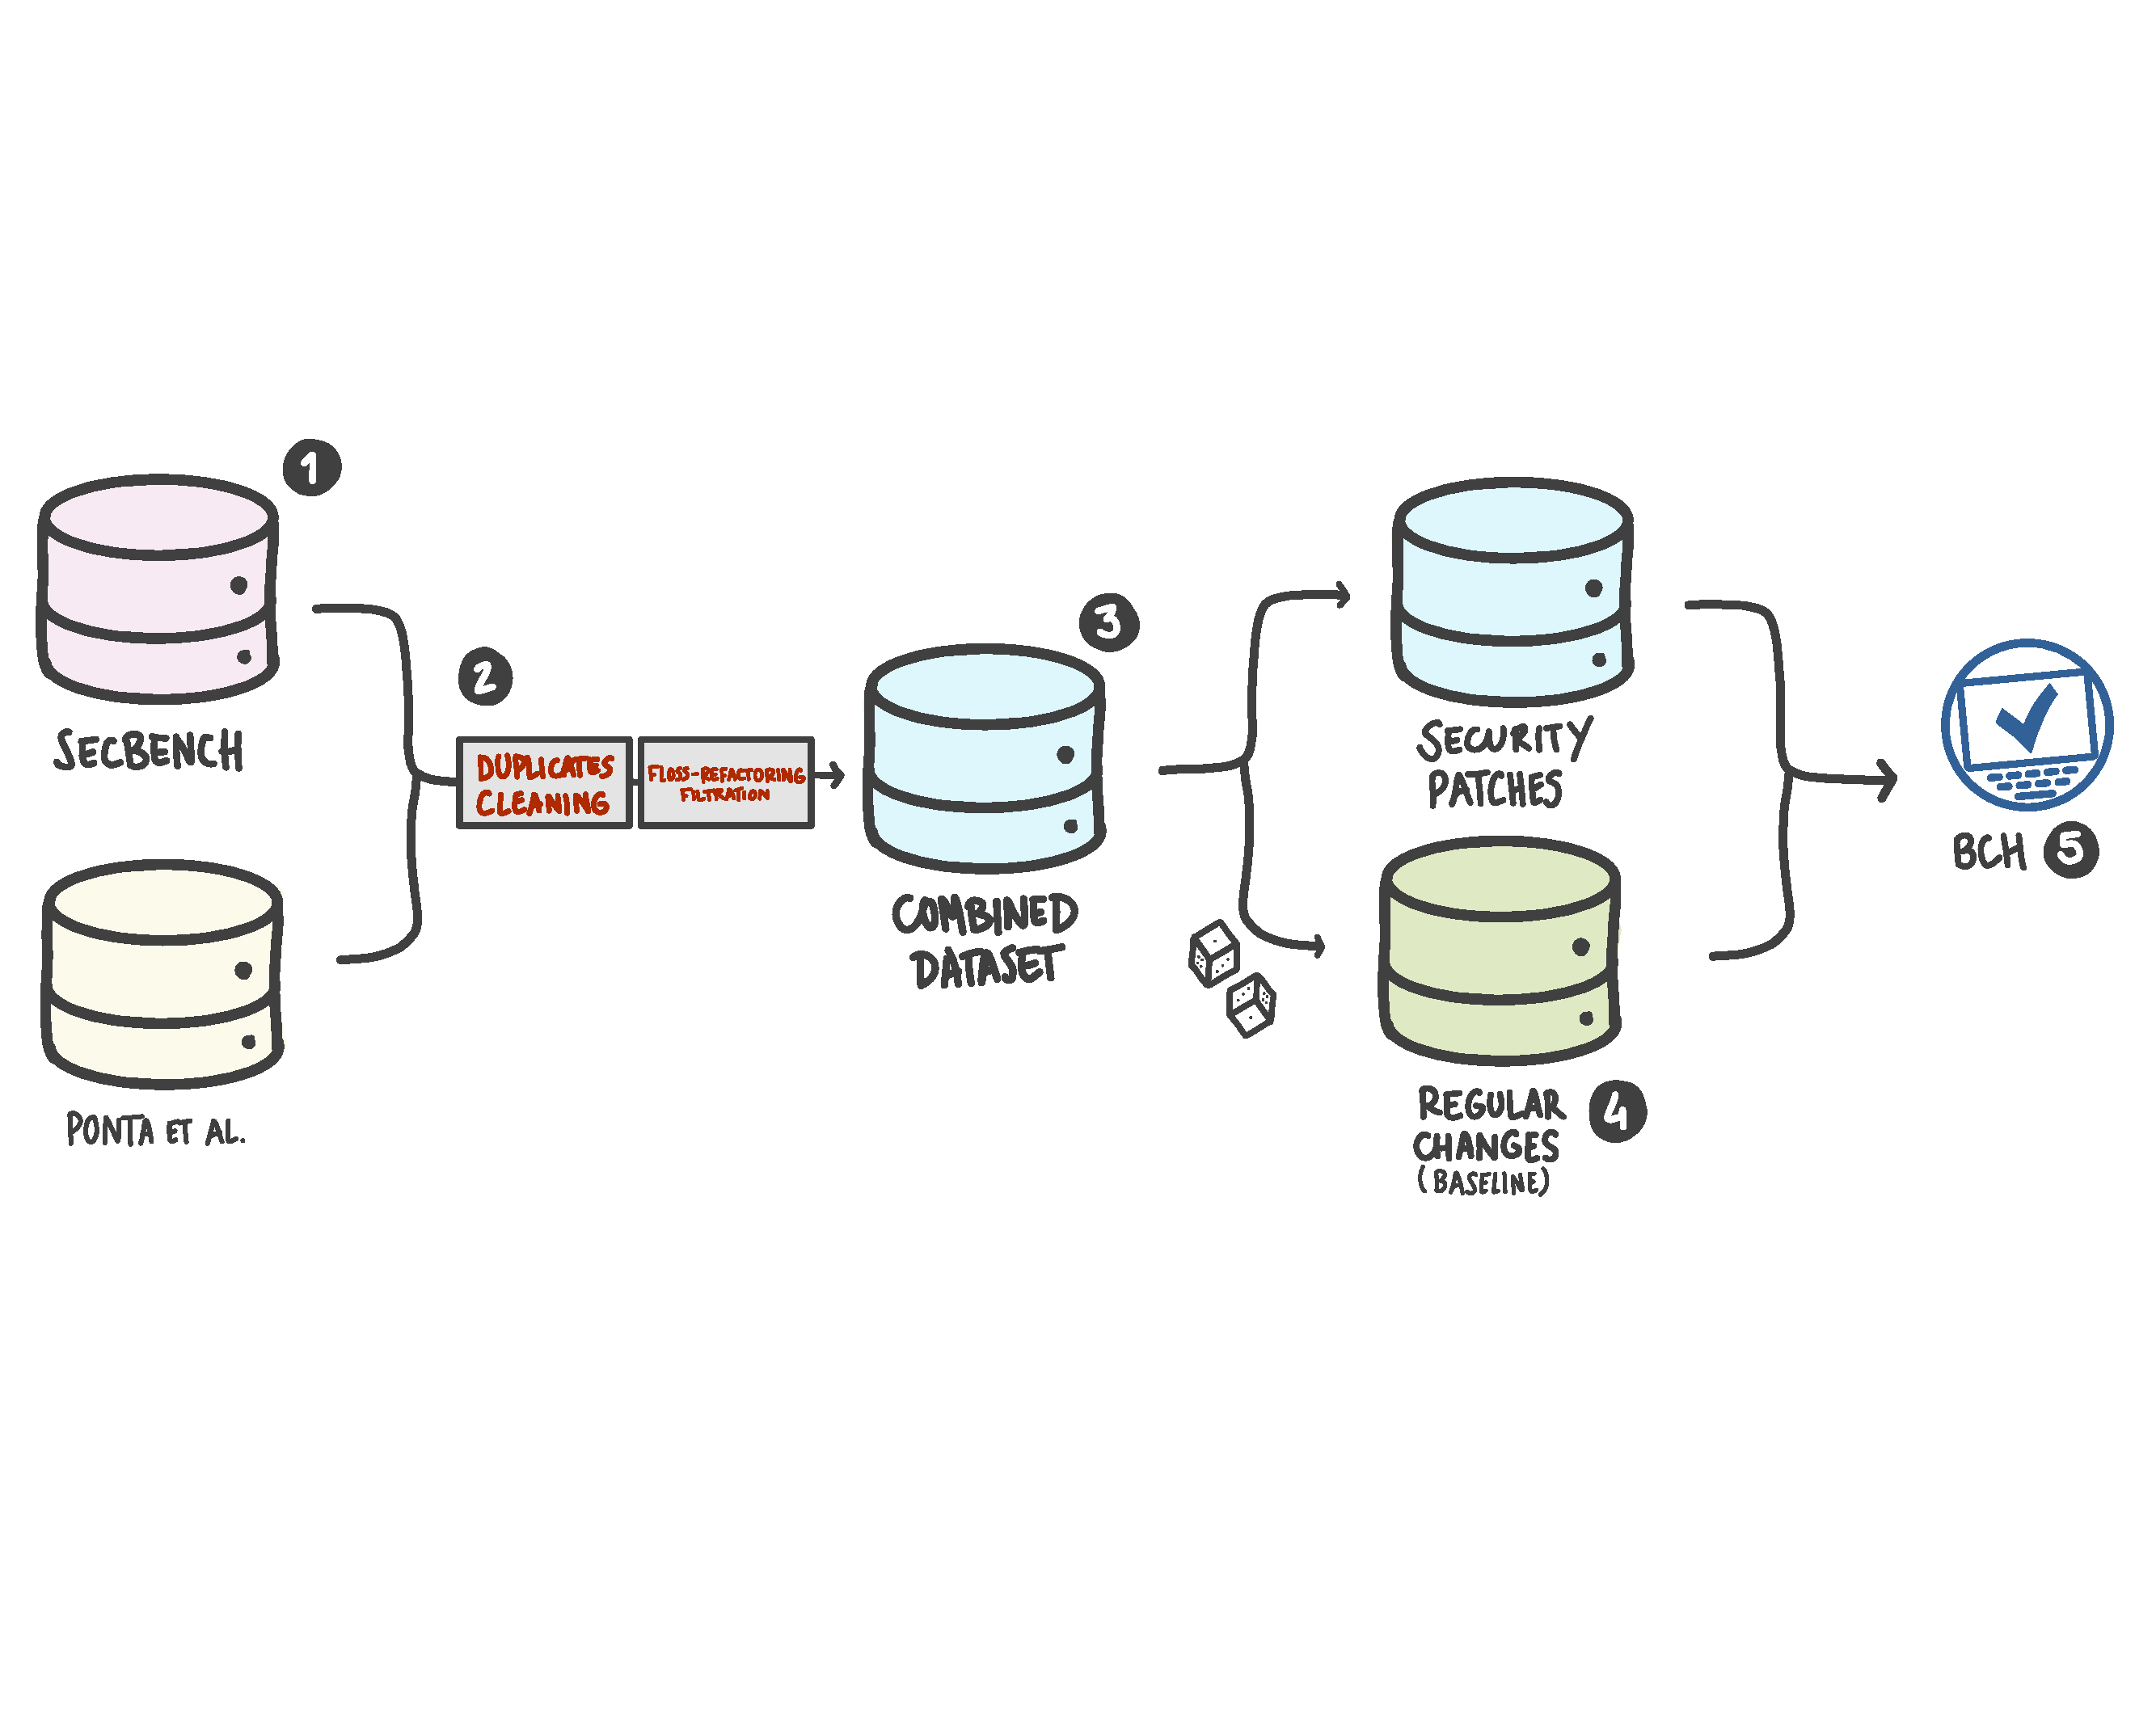
\includegraphics[width=1.1\textwidth]{figures/methodology.pdf}
  \vspace{-3cm} 
  \caption{Study Methodology}
	\label{fig:met}
	 \end{adjustwidth}
\end{figure}
%
\subsection{Datasets}
%

We use a combined dataset of $1300$ security patches which is 
the outcome of mining and manually inspecting a total of $312$ 
GitHub projects. The combined dataset integrates two different
works: SECBENCH~\cite{reis2017secbench,Reis:2017:IJSSE} and Ponta et al.~\cite{10.1109/MSR.2019.00064}.

Reis and Abreu 
($2017$) mined open-source software aiming at the extraction of 
real---created by developers---patches of security vulnerabilities 
to test and assess the performance of static analysis 
tools~\cite{reis2017secbench,Reis:2017:IJSSE} since using hand-seeded test cases or 
mutations can lead to misleading assessments of the capabilities of 
the tools~\cite{just2014mutants}. The study yielded a dataset of 
$676$ patches for $16$ different security vulnerability types, dubbed as SECBENCH. 
The vulnerability types are based on the OWASP Top $10$ of 
$2013$~\cite{oswap:2013} and OWASP Top $10$ of 
$2017$~\cite{oswap:2017}. Each test case of the dataset is a 
triplet: the commit before the patching (\emph{sha-p}), the commit responsible
for the patching (\emph{sha}), and the snippets of code that differ from one 
version to another (typically, called \emph{diffs})---where one 
can easily review the code used to fix the vulnerability. 
%
Ponta et al. ($2019$) tracked the \url{pivotal.io} website for 
vulnerabilities from $2014$ to $2019$. For each new vulnerability, 
the authors manually searched for references to commits involved in 
the patch on the National Vulnerability Database (NVD) website. 
However, $70\%$ of the vulnerabilities did not have any references 
to commits. Thus, the authors used their expertise to locate the 
commits in the repositories. This technique yielded a dataset of 
$624$ patches~\cite{10.1109/MSR.2019.00064} and $1282$ commits---one 
patch can have multiple commits assigned. To fit the dataset in our methodology, we located the 
first and last commits used to patch the vulnerability. For these 
cases, we used the GitHub API to retrieve automatically the dates of 
the commits. Then, for each patch, the group of commits was ordered 
from the oldest commit to the newest one. We assumed the last commit 
(newest one) as the fix (\emph{sha}) and the parent of the 
first commit (oldest commit) as the vulnerable version 
(\emph{sha-p}). 
%

In this study, we focus on computing the maintainability of the 
commits before and after the security patching to evaluate if its 
impact was positive, negative or none. The $1300$ patches in the 
dataset were analyzed using the BCH toolset to calculate their 
maintainability reports. Due to the limitations of BCH (in particular, 
lack of language support and project size) and the presence of
floss-refactorings, $331$ patches were tossed---explained in 
more detail in Section~\ref{sec:main_analysis}.
The final dataset used in this 
paper comprises $969$ security patches from $260$ projects. We used the 
Common Weakness Enumeration (CWE) taxonomy to classify each vulnerability. 
For instance,  the \texttt{Fix CVE-2014-1608: mc\_issue\_attachment\_get SQL injection} 
(\texttt{00b4c17}\footnote{CVE-$2014$-$1608$ details available at 
\url{https://github.com/mantisbt/mantisbt/commit/00b4c17088fa56594d85fe46b6c6057bb3421102} 
(Accessed on \today)}) is a \emph{CWE-89: Improper Neutralization of Special Elements used 
in an SQL Command ('SQL Injection')}\footnote{CWE-$89$ details available at \url{https://cwe.mitre.org/data/definitions/89.html} 
(Accessed on \today)} according to the CWE taxonomy.
We were able to classify a total of $866$ patches \Sofia{not sure why i did not classified all of them}using the CWE taxonomy
where the CWEs for $536$ patches were automatically scraped from the National 
Vulnerability Dataset (NVD); while for the other $330$ patches, the CWEs were manually 
chosen by the authors following the \emph{Research Concepts} CWE's list.

% In Table~\ref{tab:patterns}, the most prevailing categories are presented. To satisfy the Wilcoxon test size requirement, types of vulnerabilities
% with less than $20$ instances were merged in a bigger group named \textit{Miscellaneous}.

% \begin{table}[h]
% \scriptsize
% 	\caption{Guidelines to produce maintainable code}
% \begin{tabular}{L{1.1cm}L{2.1cm}L{4.3cm}}
%
% \toprule
% \textbf{Pattern} & \textbf{Name} & \textbf{Description}\\
% \midrule
%
% \textbf{CWE-89} &
%  Improper Neutralization of Special Elements used in an SQL Command/SQL Injection (23 cases) &
%  When developers do not keep untrusted data
%      separate from SQL queries. If an attacker sends a command that
%      exploits the syntax of the SQL interpreter, then SQL injection attack is possible.\\\midrule
%
% \textbf{CWE-611} &
%  Improper Restriction of XML External Entity Reference (24 cases) &
% 	XML documents are exchanged through the web containing entities with URIs
%  	that resolve to local/external files. Thus, when XML parsers are not well configured,
%  	attackers have allowed to directly those files.\\\midrule
%
%  \textbf{CWE-20} &
%  Improper Input Validation (76 cases) &
% 	When developers
%  	forget to validate the inputs of an application, attackers may have control
%  	of the control/data flow of the program.\\\midrule
%
%   \textbf{CWE-200} &
% Information Exposure (39 cases)&
% Application's logs are one way of intentional/unintentional disclosure information
%  	to attackers. Many times attackers get access to logs when sould not be authorized to.\\\midrule
%
%    \textbf{CWE-352} &
% Cross-Site Request Forgery/CSRF (22 cases)&
% Poor session tokens generation
%      and management usually allow attackers to send forged HTTP requests
%      including authentication information from the victim to the vulnerable web
%      application.\\\midrule
%
%        \textbf{CWE-264} &
% Permissions, Privileges, and Access Controls (59 cases)&
% Incorrectly
%  	    implemented functionalities related to authentication and session
%  	    management, allowing an attacker to gain access to session tokens,
%  	    passwords, keys, and other sensitive data.\\\midrule
%
%  	           \textbf{CWE-399} &
% Resource Management Errors (22 cases)&
% Resource management issues are found more frequently
%  		in programming languages that do not manage memory automatically (e.g., C/C++
%  	    and Objective-C), i.e., where developers are responsible for
%  	    handling it instead. It is one of the main causes of Denial-of-Service attacks.\\\midrule
%
%  	     	           \textbf{CWE-79} &
% Improper Neutralization of Input During Web Page Generation/Cross-site Scripting (63 cases)&
% Lack of proper validation or escaping
%  	    allows attackers to submit untrusted data to web browsers through malicious
%  	    scripts that can hijack the user sessions or redirect the user to malicious
%  	    sites.\\\midrule
%
%  	     	           \textbf{CWE-22} &
% Improper Limitation of a Pathname to a Restricted Directory/Path Traversal (37 cases) &
% When developers forget to neutralize special elements within the path names to files/directories, attackers
%  	may leverage this flaw to resolve to a location outside of the restricted directory and gain access to documents
%  	or entire repositories.\\\midrule
%
%  	 	     	           \textbf{MISC} &
% Miscellaneous (666 cases) &
% This pattern comprises
%  		several other security patches that do not have a CWE assigned and patterns that
%  		do not satisfy the Wilcoxon test size requirement of more than $20$ patches.\\
% \bottomrule
% \end{tabular}
% \label{tab:patterns}
% \end{table}

%
% \begin{itemize}
%     \item \textbf{CWE-89: Improper Neutralization of Special Elements used in an SQL Command/SQL Injection (23 cases).} When developers do not keep untrusted data
%     separate from SQL queries. If an attacker sends a command that
%     exploits the syntax of the SQL interpreter, then SQL injection attack is possible.
% %
%     \item \textbf{CWE-611: Improper Restriction of XML External Entity Reference (24 cases).}
% 	XML documents are exchanged through the web containing entities with URIs
% 	that resolve to local/external files. Thus, when XML parsers are not well configured,
% 	attackers have allowed to directly those files.
% %
%     \item \textbf{CWE-20: Improper Input Validation (76 cases).} When developers
% 	forget to validate the inputs of an application, attackers may have control
% 	of the control/data flow of the program.
% %
%     \item \textbf{CWE-200: Information Exposure (39 cases).} Application's logs are one way of intentional/unintentional disclosure information
% 	to attackers. Many times attackers get access to logs when sould not be authorized to.
% %
% 	\item \textbf{CWE-352: Cross-Site Request Forgery/CSRF (22 cases).} Poor session tokens generation
%     and management usually allow attackers to send forged HTTP requests
%     including authentication information from the victim to the vulnerable web
%     application.
% %
% 	\item \textbf{CWE-264: Permissions, Privileges, and Access Controls (59 cases).} Incorrectly
% 	    implemented functionalities related to authentication and session
% 	    management, allowing an attacker to gain access to session tokens,
% 	    passwords, keys, and other sensitive data.
% %
% 	\item \textbf{CWE-399: Resource Management Errors (22 cases).} Resource management issues are found more frequently
% 		in programming languages that do not manage memory automatically (e.g., C/C++
% 	    and Objective-C), i.e., where developers are responsible for
% 	    handling it instead. It is one of the main causes of DoS attacks.
% %
% 	\item \textbf{CWE-79: Improper Neutralization of Input During Web Page Generation/Cross-site Scripting (62 cases)} Lack of proper validation or escaping
% 	    allows attackers to submit untrusted data to web browsers through malicious
% 	    scripts that can hijack the user sessions or redirect the user to malicious
% 	    sites.
% %
% 	\item \textbf{CWE-22: Improper Limitation of a Pathname to a Restricted Directory/Path Traversal (37 cases).}  When developers forget to neutralize special elements within the pathnames to files/directories, attackers
% 	may leverage this flaw to resolve to a location outside of the restricted directory and gain access to documents
% 	or entire repositories.
% %
% 	\item \textbf{Miscellaneous (673 cases)} This pattern comprises
% 		several other security patches that do not have a CWE assigned and patterns that
% 		do not satisfy the Wilcoxon test size requirement of more than $20$ patches.
% \end{itemize}
%
\subsection{Security Patches vs. Regular Changes}
%
Previous studies attempted to measure the impact of regular changes 
on open-source software maintainability~\cite{HEGEDUS2018313}. 
However, there is no previous work focused on comparing the impact 
of security patches with regular changes on maintainability---only
with bug-fixes~\cite{10.1145/3133956.3134072}.
We analyze the maintainability of regular changes---changes not 
related to security patches---and, use them as a baseline.
The baseline dataset is generated from the security commits dataset, i.e.,
for each security commit in the dataset we collect a random regular
change from the same project. We created two different baselines: 
\textit{random-baseline},
considering random changes and all their characteristics; and,
\textit{size-baseline}, considering also random changes
but with the same size as security patches.

\subsubsection{Size-Baseline} 

As for the security patches, for each regular change or refactoring, we also 
need the commit performing the regular change (\emph{sha-reg}) and version of 
the software before the change (\emph{sha-reg-p}). For each security patch, a 
\emph{diff} with an approximate 
size was fetched to a regular change. Due to the complexity of some patches, it was not possible 
to find patches with the exact number of added and deleted lines. 
Our search uses the security patch \emph{diff} to look for a 
\emph{diff} of the same size. The algorithm integrates the following 
steps:

\begin{enumerate}
\item Calculates the \emph{diff} between the security patch commit 
(\emph{sha}) and its parent (\emph{sha-p}).
\item Selects a random commit from the project (\emph{sha-reg}).
\item Calculates the \emph{diff} between the random commit (\emph{sha-reg}) 
and its parent (\emph{sha-reg-p}).
\item Checks if the size from the regular change has the 
same/approximated size to the security patch.
\end{enumerate}

The pair of the random commit and its parent is accepted if the 
\emph{diff} size fits in the range size. This range widens every 
$10$ attempts to search for a change with the same size. We 
originate the regular changes from the security commits to ensure 
that differences in maintainability are not a consequence of 
characteristics of different projects.

\subsubsection{Random-Baseline} 

As for the security patches, for each regular change or refactoring, we also 
need the commit performing the regular change (\emph{sha-reg}) and version of 
the software before the change (\emph{sha-reg-p}). For each security patch, 
a random commit is selected from the the project (\emph{sha-reg}).

\subsection{Why Bettter Code Hub?}

SIG---the company behind BCH--has been helping business and technology 
leaders drive their organizational 
objectives by fundamentally improving the health and security of 
their software applications for more than $20$ years. The
inner-working of their SIG-MM model---which is the one behind BCH---was 
scientifically proven~\cite{4335232,5609747,6113040,baggen2012}.
BCH not only considers security on their maintainability model~\cite{6616351}
but also integrates a total of $10$ different code metrics; and, 
code metrics were empirically validated in previous 
work~\cite{Bijlsma:2012:FIR:2317098.2317124,8530041,8919169,8785997}.

As BCH there are other tools that do the same kind of code analysis.
Two examples are Kiuwan and SonarCloud. Kiuwan is not free, their 
inner-workings do not seem to be published anywhere and there is
no clear list of metrics available---we inspected their datasheet.
SonarCloud is free but uses only $4$ of the guidelines (duplication,
size, complexity and code smells) that BCH considers. It also scores 
maintainability. In the following table, we
present a brief comparison between BCH and SonarCloud:

\Sofia{Currently building a script to retrieve the SonarCloud results}


\subsection{Maintainability Analysis}\label{sec:main_analysis}

In this research, we follow a very similar methodology to the one 
presented in previous work on the maintainability of energy-oriented 
fixes~\cite{8919169}. The inner-workings of BCH were proposed
originally in 2007~\cite{4335232} and suffer refinements later~\cite{5609747,6113040,baggen2012}. 
As said before, the web-based source code 
analysis service \emph{Better Code Hub} (BCH) is used to collect the 
maintainability reports of the patches of each project. 
Table~\ref{tab:guidelines} presents the $10$ guidelines proposed
by BCH's authors for delivering software that is not difficult to
maintain~\cite{Visser:2016:OREILLY} and, maps each guideline to the 
metric calculated by BCH. Theses guidelines are calculated using the 
metrics presented in~\cite{criteria:2017} and are also briefly 
explained on Table~\ref{tab:guidelines}. 
During each guideline evaluation, the tool determines the compliance 
towards one guideline by establishing limits for the percentage of 
code allowed to be in each of the $4$ risk severity levels
(\emph{low risk}, \emph{medium risk}, \emph{high risk}, and 
\emph{very high risk}). If the project does not violate those 
thresholds, then the BCH considers that the code is compliant with 
a guideline. These thresholds are determined by BCH using their own
data/experience---using open-source and closed software systems. If 
a project is compliant with a guideline, it means that it is at 
least $65\%$ better than the software used by BCH to calculate the 
thresholds\footnote{Check the answer to \emph{How can I adjust the 
threshold for passing/not passing a guideline?} at
\url{https://bettercodehub.com/docs/faq} (Accessed on \today{})}.

\begin{table}[h]
\centering
\scriptsize
	\caption{Guidelines to produce maintainable code. \Sofia{Still need to add more references}}
\begin{tabular}{L{2cm}L{4.5cm}L{4cm}}

\toprule
\textbf{10 Guidelines} & \textbf{Description} & \textbf{Metric}\\
\midrule

\textbf{Write Short Units of Code} & Limit code units to $15$ LOCs because smaller
 units are easier to understand, reuse and test them & \textbf{Unit Size:} \% of 
 LOCs within each unit~\cite{criteria:2017} \\\midrule

\textbf{Write Simple Units of Code} & Limit branch points to $4$ per unit because
it makes units easier to test and modify & \textbf{McCabe Complexity:} \# of decision 
points~\cite{1702388,criteria:2017}\\\midrule

\textbf{Write Code Once} & Do not copy code because bugs tend to replicate at
multiple places (inefficient and error-prone) & \textbf{Duplication:} \% of redundant 
LOCs~\cite{criteria:2017}\\\midrule

\textbf{Keep Unit Interfaces Small} & Limit the number of parameters to at most
$4$ because it makes units easier to understand and reuse & \textbf{Unit Interfacing:} 
\# of parameters defined in a signature of a unit~\cite{criteria:2017} \\\midrule

\textbf{Separate Concerns in Modules} & Avoid large modules because changes in
loosely coupled databases are easier to oversee and execute & \textbf{Module Coupling:} \# of
incoming dependencies~\cite{criteria:2017} \\\midrule

\textbf{Couple Architecture Components Loosely} & Minimize the amount of code
within modules that are exposed to modules in other components & \textbf{Component Independence:} 
\% of code in modules classified as hidden~\cite{criteria:2017}\\\midrule

\textbf{Keep Architecture Components Balanced} & Balancing the number of
components ease locating code and allow for isolated maintenance & \textbf{Component Balance:} 
Gini coefficient to measure the inequality of distribution between components~\cite{criteria:2017} \\\midrule

\textbf{Keep your code base Small} & Reduce and avoid the system size because
small products are easier to manage and maintain & \textbf{Volume:} \# of LOCs converted 
to man-month/man-year~\cite{criteria:2017} \\\midrule

\textbf{Automate Tests} & Test your code base because it makes development
predictable and less risky & \textbf{Testability:} Ratings aggregation $-$ unit 
complexity, component independence and volume~\cite{Visser:2016:OREILLY}
 \\\midrule

\textbf{Write Clean Code} & Avoid producing software with code smells because
it is more likely to be maintainable in the future & \textbf{Code Smells:} 
\# of Occurrences~\cite{Visser:2016:OREILLY} (e.g., magic constants and long 
identifier names) \\
\bottomrule
\end{tabular}
\label{tab:guidelines}
\end{table}

Figure~\ref{fig:bchrep} shows an example of the report provided by BCH 
for a project after finishing its evaluation. The example
refers to the OpenSSL CVE-$2016$-$6304$ vulnerability patch---
as described by Section~\ref{sec:motivation}. This version of 
OpenSSL only complies with $1$ out of $10$ guidelines: \emph{Write 
Clean Code}.

\begin{figure}[h]
 	\centering 	
	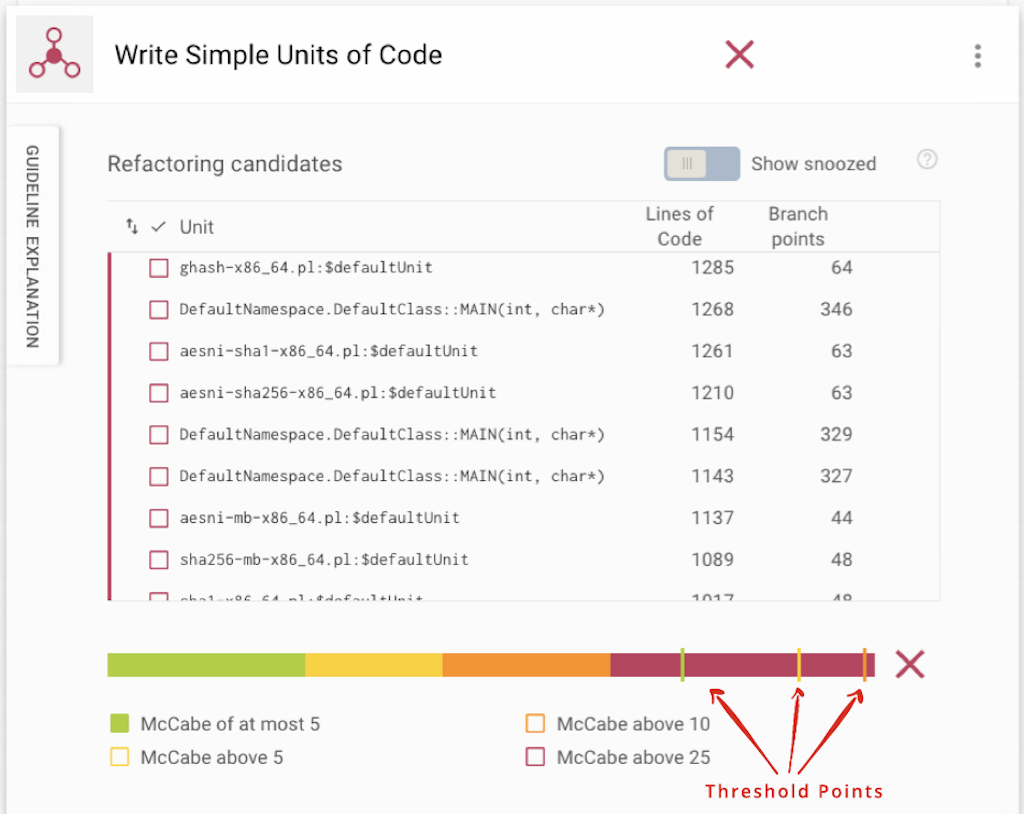
\includegraphics[width=0.8\textwidth]{figures/bch_report.png}
 	\caption{Maintainability report of OpenSSL's CVE-$2016$-$6304$ 
	vulnerability patch for the guideline \emph{Write Simple Units 
	of Code} provided by \emph{Better Code Hub}. This version of 
	OpenSSL does not comply with the guideline in the example since 
	the bars do not reach the threshold points. This example only 
	complies with $\sfrac{1}{10}$ guidelines (\emph{Write Clean 
	Code}).}
	\label{fig:bchrep}
\end{figure}

SIG defines \emph{Units} as the smallest groups of code that can be 
maintained and executed independently~\cite{Visser:2016:OREILLY} 
(e.g., methods and constructors in Java). One of the guidelines with 
which the project does not comply is the one presented in the report 
(cf. Figure~\ref{fig:bchrep}): \emph{Write Simple Units of Code}. BCH 
analyzes this guideline based on the McCabe 
Complexity~\cite{1702388} to calculate the number of branch points 
of a method. The bar at the bottom of the figure represents the top 
$30$ units that violate the guideline, sorted by severity. The 
different severities of violating the guideline are indicated using 
colors, and there is a legend to help to interpret them. The green 
bar represents the number of compliant branch points per unit 
(\emph{at most $5$}), i.e., the number of units are compliant with 
ISO $25010$~\cite{iso:2011}. Yellow, orange and red bars represent 
units that do not comply with medium (\emph{above $5$}), high 
(\emph{above $10$}) and very high (\emph{above $25$}) severity 
levels. In the bar, there are marks that pinpoint the compliance 
thresholds for each severity level. If the green mark is somewhere 
in the green bar it means it is compliant with a low level of
severity.

Aiming to analyze the impact of security patches, we use BCH to compute 
the maintainability of two different versions of the project 
(cf. Figure~\ref{fig:commit}):

\begin{itemize}
	\item $v_{s-1}$, the version containing the security flaw, i.e., 
	before the patch (\emph{sha-p});
	\item $v_{s}$, the version free of the security flaw, i.e., 
	after the patch (\emph{sha});
\end{itemize}

\begin{figure}[h]
 	\centering 	
	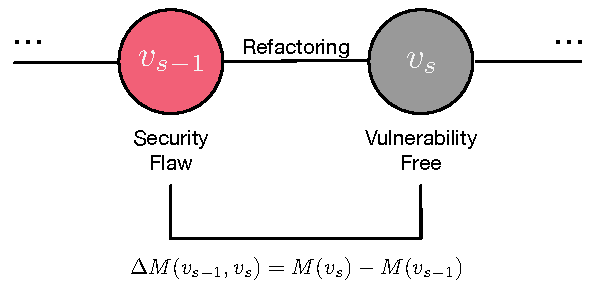
\includegraphics[width=0.5\linewidth]{figures/commit.pdf}
 	\caption{Maintainability difference for security commits.}
	\label{fig:commit}
\end{figure}

The same approach is used to analyze the impact of regular 
changes. Security patches can be performed through one commit, 
several consecutive commits, or commit(s) interleaved with more 
programming activities (floss-refactoring). Only $10.7\%$ of the data points 
of our dataset involve more than one commits, the other
$89.3\%$ of the cases are single-commit patches. We manually 
inspected these cases and $23$ floss-refactorings were identified 
and disregarded since it would not be fair to measure the 
maintainability of these cases where other programming activities 
are involved.

For projects with large codebases, the results retrieved for 
\emph{Keep Your Codebase Small} were not viable because they 
retrieved values above the limit set by BCH ($20$ Person-years). The 
\emph{Automated Tests} guideline was also not considered since the 
tool does not contemplate two of the most important techniques to 
security testing: vulnerability scanning and penetration testing. 
Instead, it only contemplates unit testing. Due to BCH limitations, 
we detected $308$ data points that retrieved incorrect overall 
calculations. Those data points were disregarded from the study.

The BCH tool does not compute the final score that our study needs 
to compare maintainability amongst different project versions. For 
this, we follow previous work on measuring the impact of 
energy-oriented patches~\cite{8919169}. Cruz et al. ($2019$) 
proposed an equation to capture the distance between the current 
state of the project and the standard thresholds calculated by the 
BCH based on the insights provided in~\cite{Olivari:2018}. The 
equation provided in~\cite{8919169} considers that the size of 
project changes does not affect the maintainability and that the 
distance to lower severity levels is less penalized than to the
thresholds in high severity levels.

% 	thresholds in high severity levels
% 	difference between two versions
% The equation considers the following:
% \begin{itemize}
% 	\item \textbf{Size of project changes does not affect the maintainability
% 	difference between two versions, $\Delta M (v_{s-1},v_{s}) = M(v_{s}) - M(v_{s-1})$.} We
% 	aim at evaluating security patterns occurring in different projects similarly.
% 	Thus, the derived metric uses the \textit{raw} number of lines of code rather
%   percentages for normalization purposes.
% 	\item \textbf{Distance to lower severity levels is less penalized than to the
% 	thresholds in high severity levels.} Severity level weights based on the
% 	severity level to count lines of code that violate maintainability guidelines.
% \end{itemize}


Given the violations for the BCH guidelines, the maintainability 
score is computed $M(v)$ as follows:

\begin{equation}
    M(v) = \sum_{g \in G}^{} M_{g}(v)
\end{equation}

\noindent
where $G$ is the group of maintainability guidelines from BCH
(Table~\ref{tab:guidelines}) and $v$ is the version of the software 
under evaluation. $M(v) < 0$ indicates that version $v$ is violating 
(some of) the guidelines, while $M(v) > 0$ indicates that version 
$v$ is following the BCH guidelines. The maintenance for the 
guideline $g$, $M_g$ for a given version of a project is computed as 
the summation of the compliance with the maintainability guideline 
for the given severity level (medium, high, and very high).
The compliance for a severity level is calculated based on previous 
work, which calculates the number of lines of code that comply and 
not comply with the guideline at a given severity 
level~\cite{8919169}. In our analysis, we compute the difference of 
maintainability between the security commit ($v_{s}$) and its parent 
commit ($v_{s-1}$), as illustrated in Figure~\ref{fig:commit}. Thus, 
we can determine which patches had a positive, negative, or null 
impact on the project maintainability. 

% The compliance $C$ for a given severity
% level $l$ is derived by:
%
% \begin{equation}\label{eq:3}
%     C(l) = LOC_{compliant}(l) - w(l) * LOC_{\neg compliant}(l)
% \end{equation}
%
% \noindent
% where $LOC_{compliant}(l)$ are the lines of code that comply with the guideline
% at the given severity level $l$, $LOC_{\neg compliant}(l)$ are the lines of code
% that do not comply with the guideline at the given severity level $l$ and $w(l)$
% is the weight factor to heighten the impact of non-compliant lines in comparison to
% compliant lines. Finally, the term $w(l)$ is calculated as follows:
%
% \begin{equation}
%     w(l) = \frac{1 - \theta(l)}{\theta(l)}
% \end{equation}
%
% \noindent
% where $\theta(l)$ is the threshold in percentage of the lines of code that are
% accepted to be non-compliant with the guideline for the severity level $l$. This
% is a standard value defined by BCH. In other words, the factor $w$ is used in
% Equation~\ref{eq:3} to highlight the lines of code that are not complying with
% the guideline. Then, we compute the difference of maintainability between the
% security commit ($v_{s}$) and its parent commit ($v_{s-1}$), as illustrated in
% Figure~\ref{fig:commit}.

\subsection{Statistical Validation}\label{sec:statsval}
%
To validate the maintainability differences in different groups of 
commits (e.g., baseline and security commits), we use the Paired 
Wilcoxon signed-rank test with the significance level $\alpha = 
0.05$~\cite{10.2307/3001968}. In other words, we test the null 
hypothesis that the maintainability difference between pairs of 
versions $v_{s-1}$, $v_s$ (i.e., before and after a security-commit) 
come from the same distribution. Nevertheless, this test 
has a limitation: it does not consider the groups of commits with a 
zero-difference maintainability. In $1959$, Pratt provided an 
improvement to the test to solve this issue making the test more 
robust. Thus, we use a version of the Wilcoxon test that 
incorporates the cases where maintainability is different from 
zero~\cite{10.2307/2282543}. The Wilcoxon test requires a 
distribution size of at least $20$ instances. To understand the 
effect-size, as advocated by the Common-language effect 
sizes, we compute the mean difference, the median of 
the difference, and the percentage of cases that reduce 
maintainability~\cite{graw:1992}.
%

\section{Results \& Discussion}\label{sec:results}

This study evaluates a final total of $969$ security patches from $260$ 
distinct open-source projects. This section 
reports and discusses the results for each research question.
%

\textit{\textbf{RQ1: What is the impact of security patches on the
maintainability of open-source software?}} In \emph{RQ1}, we 
report and discuss the impact of patches on open-source software 
maintainability under four groups: guideline, overall score, 
severity and programming language.

\textbf{Guideline/Metric:} Each patch performs a set of changes
on the source code of the software. These changes may have a 
different impact on the guidelines/metrics used to measure software 
maintainability. Figure~\ref{fig:guidelines} shows the impact of 
security patches on each guideline individually and the average 
impact on all guidelines together ($M(v)$). Under each guideline, it 
is stated the metric used for the calculations. For instance, for the 
\emph{Write Short Units of Code} guideline, the metric used is 
\emph{Unit Size}. Table~\ref{tab:guidelines} describes in more 
detail the metrics behind the guidelines. For each type of 
guideline, a swarmplot is presented to show the variability and 
dispersion of the results alongside the number of absolute and 
relative cases of each impact. Next to each type of guideline, it is 
presented the mean ($\overline{x}$) and median (M) of the 
maintainability difference and the p-value resulting from the Paired 
Wilcoxon signed-rank test. $M(v)$ is not a guideline but rather the 
average impact of all guidelines. Each point of the plot represents 
the impact of a security patch on software maintainability. Red, 
means the impact was negative, i.e., the patch harmed 
maintainability. Yellow, means the patch did not have any kind of 
impact on maintainability. Green, means the impact was positive, i.e., 
the patch improved software maintainability.

 \begin{figure}[htp]
     \begin{adjustwidth}{-1cm}{-1cm}  
  	\centering
  	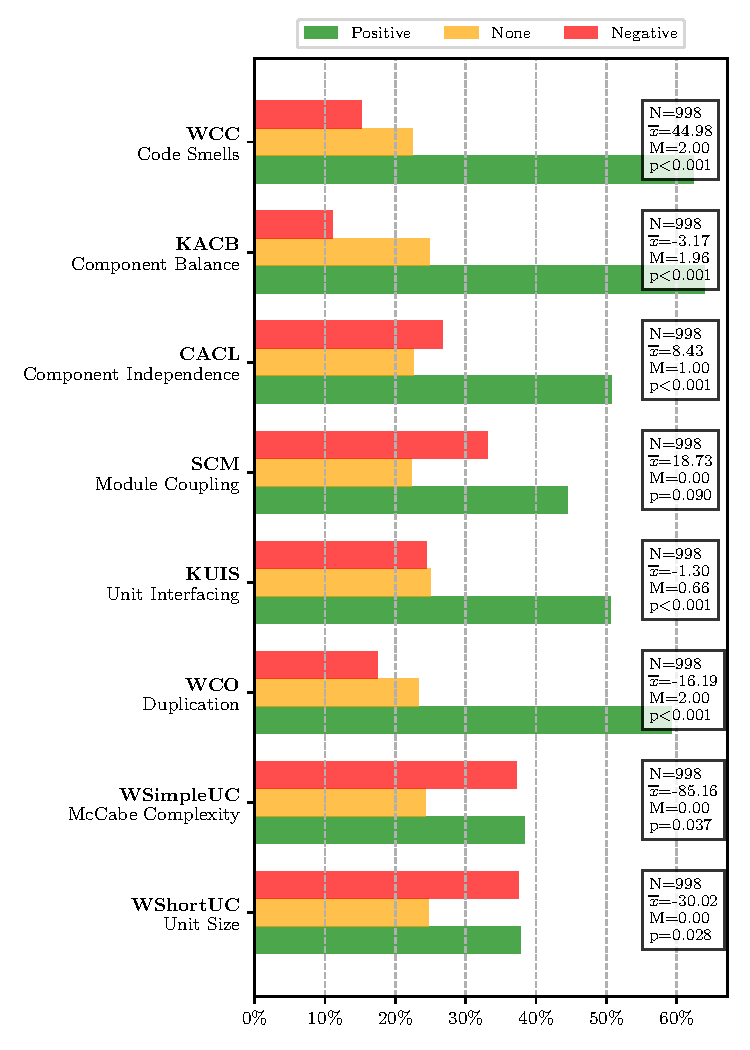
\includegraphics[width=0.9\textwidth]{figures/main_per_guideline.pdf}
    \end{adjustwidth}
	
  	\caption{Impact of the security patches per guideline and overall mean, $M(v)$. 
	Each point of the plot represents the impact of a security patch on software 
	maintainability. Red, means the impact was negative, i.e., the patch 
	harmed maintainability. Yellow, means the patch did not have any 
	kind of impact on maintainability. Green, means the impact was 
	positive, i.e., the patch improve software maintainability. For instance, in the 
	\emph{Write Short Units of Code} guideline, $38.29\%$ of 
	security patches harmed software maintainability; $23.53\%$ of 
	security patches had no impact on maintainability; and, 
	$38.18\%$ of security patches actually improved software 
	maintainability.}
 	\label{fig:guidelines}	
 \end{figure}
 
 \begin{figure}[htp]
  	\centering 	 	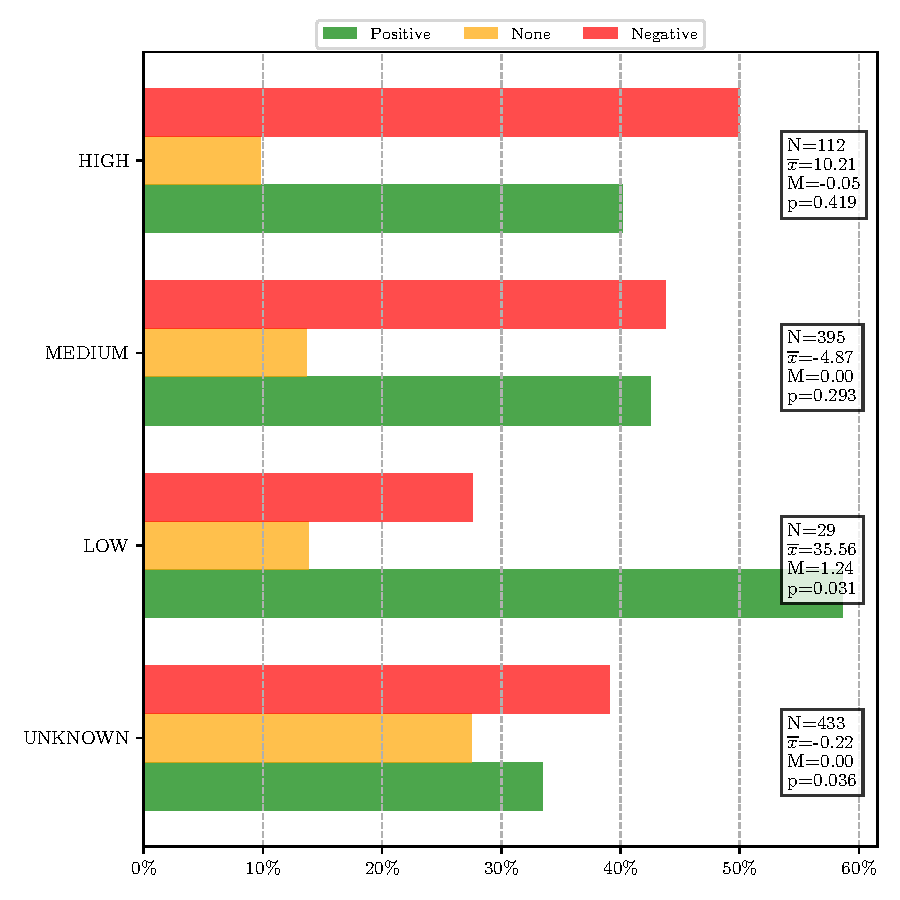
\includegraphics[width=0.65\textwidth]{figures/main_per_severity.pdf}
  	\caption{Maintainability difference by vulnerability severity.}
 	\label{fig:severity}
 \end{figure}

Regarding the impact of security patches per guideline, we 
observe that $38.7\%$ of patches have more cases where the impact is 
positive---where maintainability increases. However, we also 
see that patching vulnerabilities has a very significant number of 
negative cases per guideline---between $10\%$ and $40\%$. 
\emph{Write Short Units of Code} ($38.3\%$), \emph{Write Simple 
Units of Code} ($37.9\%$), and \emph{Separate Concerns in Modules} 
($33.8\%$) seem to be the most negatively affected guidelines. This 
may imply that developers when patching vulnerabilities have a hard 
time to design/implement solutions that continue to respect the 
limit bounds of branch points and function/module sizes that are 
recommended by coding practices. Still on respecting bound limits, 
developers also seem to not consider the limit of $4$ parameters per 
function for the \emph{Keep Unit Interfaces Small} guideline 
required by BCH, in $24.8\%$ of the cases. This guideline is usually
violated when the patch requires to input new information to a 
function/class and developers struggle to use the \emph{Introduce 
Parameter Object} patch pattern. Results do not provide statistical 
significance to the \emph{Separate Concerns in Modules} guideline, 
i.e., results should be read carefully. 

Software architecture is also affected while patching 
vulnerabilities. Both \emph{Couple Architecture Component Loosely} 
and \emph{Keep Architecture Components Balanced} guidelines suffer a 
negative impact of $26.9\%$ and $11.0\%$, respectively. Component 
independence and balance are important to make it easier to find the 
source code that developers want to patch/improve and to understand 
how the high-level components interact with others. However, results 
may imply that developers forget to use techniques such as 
encapsulation to hide implementation details and make the system 
more modular.

The \emph{Write Code Once} guideline results show that duplicated 
code increased in $171$ ($17.7\%$) of the patches. Software systems 
typically have $9\%$-$17\%$ of cloned code~\cite{5773403}. Previous 
work showed a correlation between code smells and code
duplication~\cite{7476787} which may also be reflected in the 
\emph{Write Clean Code} guideline results. BCH reported new code 
smells for $145$ ($15.0\%$) patches which according to previous work 
may harm software security since some of these new code smells may 
be new vulnerabilities~\cite{8819456}. Thus, while developers 
tend to ignore patch techniques such as the \emph{Replace Method 
with Method Object} technique, they may also be introducing new 
software vulnerabilities and, consequently, harm the market value 
and economy of companies~\cite{4267025}.

\textbf{Overall Score ($M(v)$):} 
Although overall patching vulnerabilities has a less negative impact
on software maintainability guidelines, this is not reflected in the 
average impact of all guidelines ($M(v)$) as we can see in 
Figure~\ref{fig:guidelines}. Remember that each point of the plot 
represents the impact of a security patch on software 
maintainability. Red, means the impact was negative, i.e., the patch 
harmed maintainability. Yellow, means the patch did not have any 
kind of impact on maintainability. Green, means the impact was 
positive, i.e., the patch improved software maintainability.
The $M(v)$ plot show that $406$ ($41.9\%$) cases have a negative 
impact on software maintainability. While $188$ ($19.4\%$) cases 
have no impact at all and $375$ ($38.7\%$) have a positive impact on 
software maintainability. The larger number of negative cases may be 
explained by guidelines with higher concentrations of negative 
cases with higher amplitudes, such as \emph{Write Short Units of 
Code}, \emph{Write Simple Units of Code} and \emph{Separate Concerns 
in Modules}---more red points on the left, being $0$ the reference point.
The resulting p-value of the Paired Wilcoxon signed-rank test for $M(v)$ 
is $0.044$ (cf. Figure~\ref{fig:guidelines}). Since the p-value is 
below the significance level of $0.05$, we argue that security patches 
may have a negative impact on the maintainability of open-source software.


\textbf{Severity:} Some of the vulnerabilities are identified with 
\emph{Common Vulnerabilities and Exposure} (CVE) entries. We 
leveraged the \emph{National Vulnerability Database} (NVD) website 
to collect their severity levels. In total, we retrieved severity 
scores for $536$ vulnerabilities: $112$ \emph{High}, $395$ 
\emph{Medium} and $29$ \emph{Low}. Figure~\ref{fig:severity} 
presents the impact of security patches per severity level on the 
maintainability of open-source software. We observe that patches for 
\emph{High} ($50.0\%$) and \emph{Medium} ($43.8\%$) severity 
vulnerabilities hinder more the maintainability of software than 
\emph{Low} ($27.6\%$) severity vulnerabilities. Again, patches have 
a considerable negative impact on software maintainability---between 
$20\%$ and $50\%$. Statistical significance was retrieved only for 
\emph{Low} severity vulnerabilities, i.e., \emph{Low} severity 
vulnerabilities may have more cases where software maintainability was improved than the 
other severity levels. However, results should not be disregarded 
because they seem to confirm the 
assumption that higher severity vulnerabilities patches may have a 
more negative impact on maintainability and, consequently, that high/medium 
severity vulnerabilities may need more attention than low severity while 
patching vulnerabilities.


\begin{figure}[htp]
  \centering
  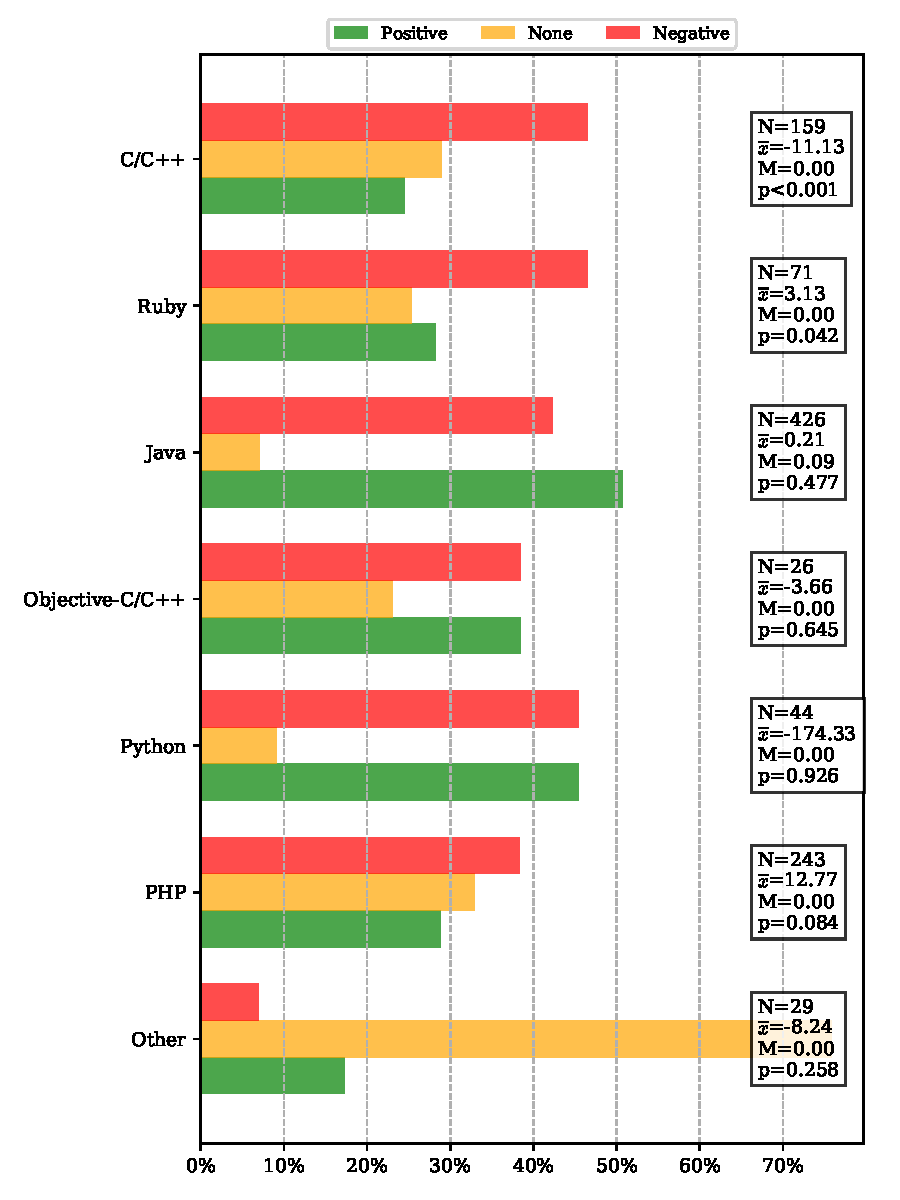
\includegraphics[width=0.6\textwidth]{figures/main_per_language.pdf}
  \caption{Maintainability difference by programming language.}
  \label{fig:lang_main}    
\end{figure}

\begin{figure*}[htp]
  \centering
  \subfigure[Maintainability difference by first-level weaknesses from the 
  \textit{Research Concepts} list on Common Weakness Enumeration (CWE)]{
  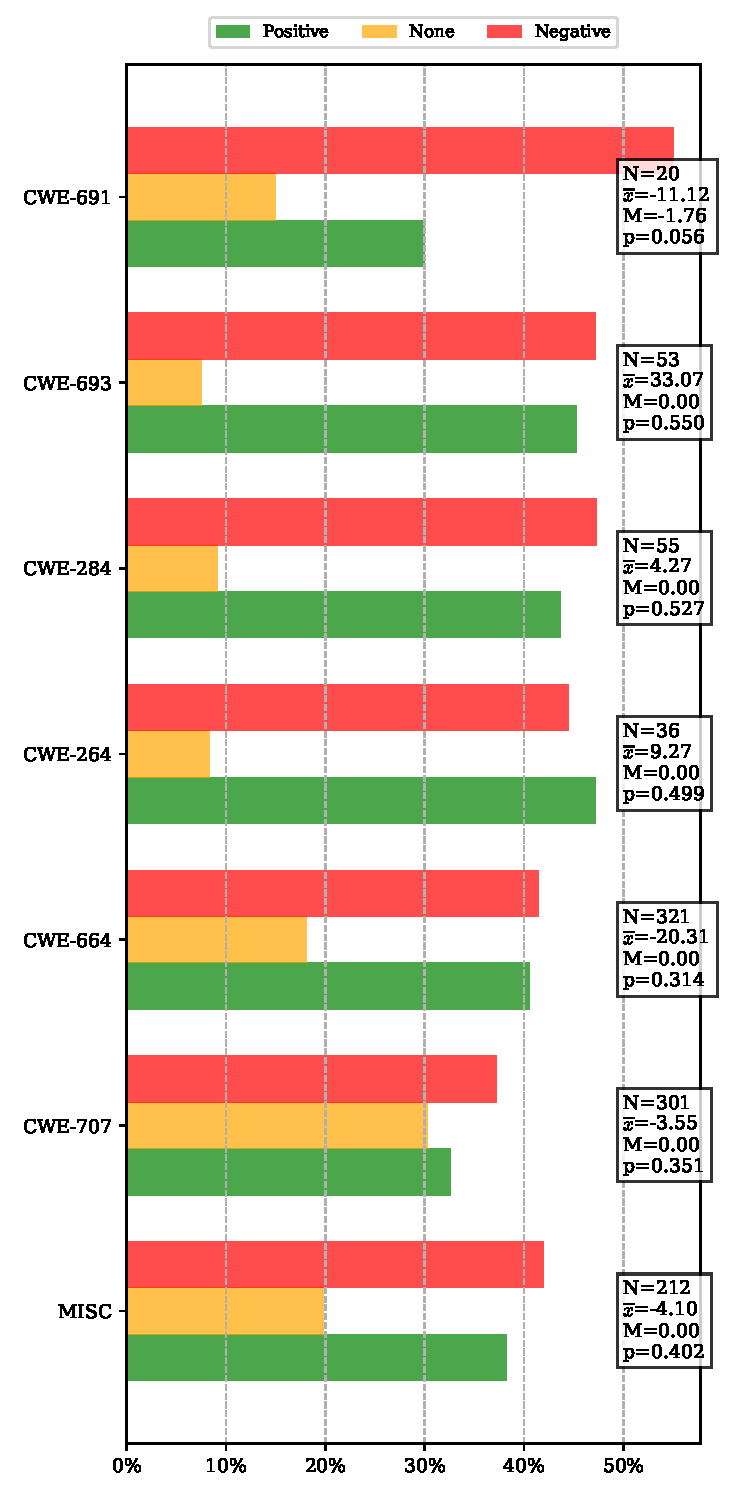
\includegraphics[scale=0.4]{figures/main_per_cwe.pdf}}\quad\quad
  \subfigure[Maintainability difference by sub-weaknesses of the 
  \textit{Improper Neutralization} Weakness (CWE-707)]{
  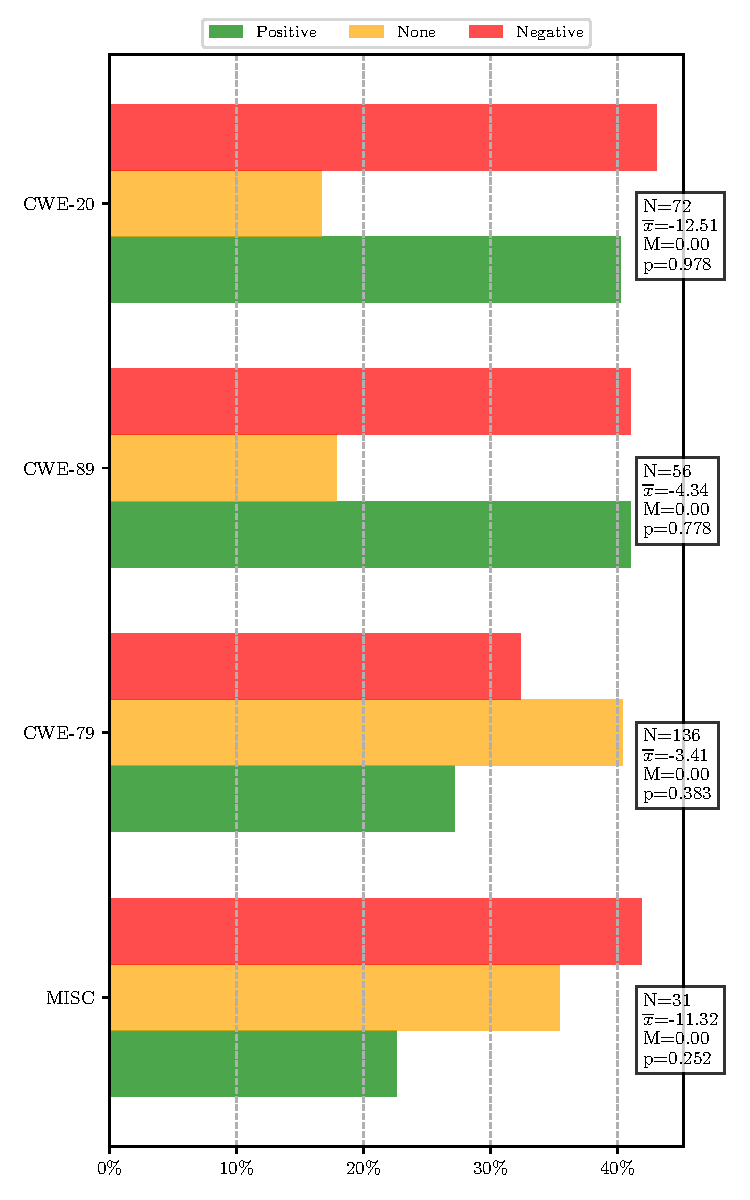
\includegraphics[scale=0.4]{figures/main_per_cwe_spec_707.pdf}}\quad\quad
    \subfigure[Maintainability difference by sub-weaknesses of the 
	\textit{Improper Control of a Resource Through its Lifetime} Weakness (CWE-664)]{
	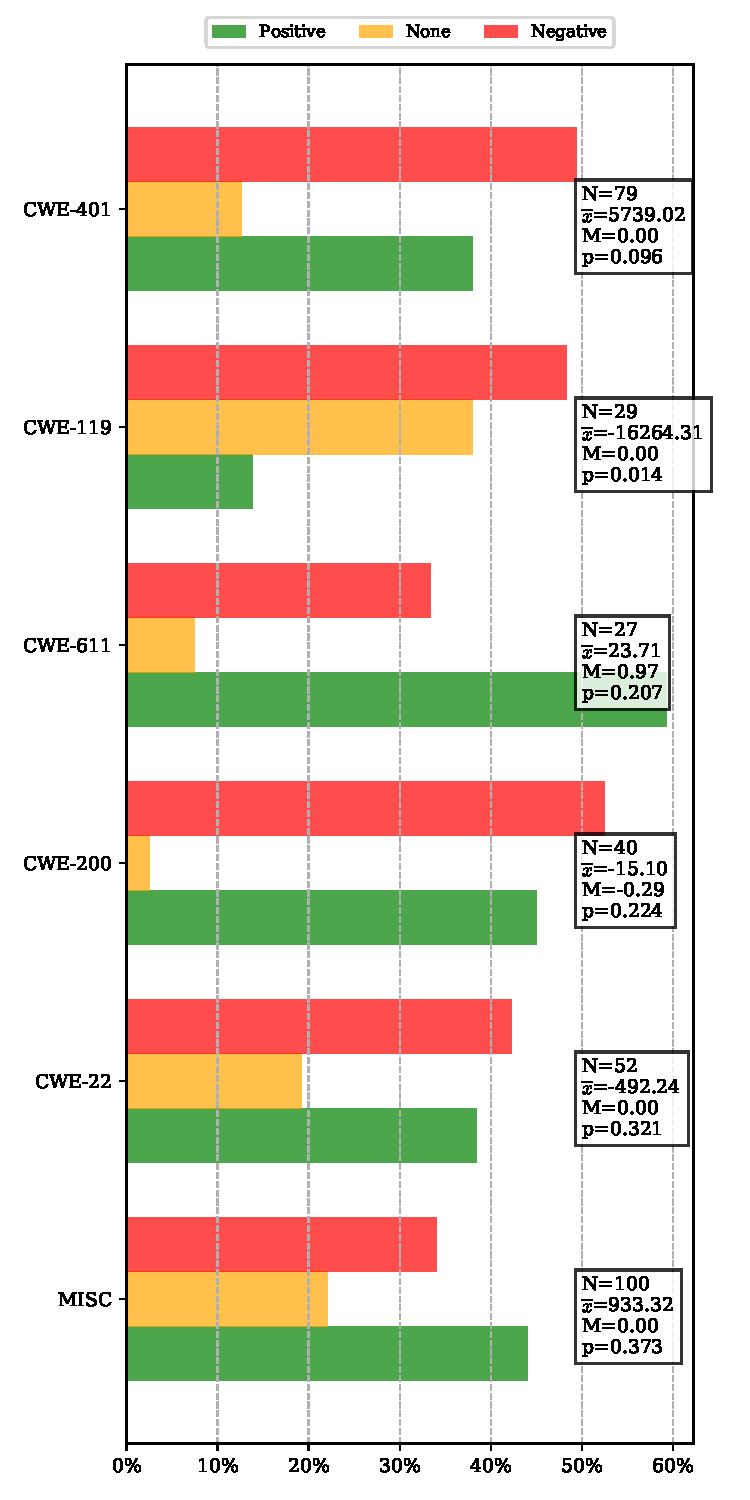
\includegraphics[scale=0.4]{figures/main_per_cwe_spec_664.pdf}}
    \caption{Maintainability difference per weakness.}
	\label{fig:pat}
\end{figure*}

\textbf{Programming Language:} The impact on software maintainability per programming 
language was also analyzed (Figure~\ref{fig:lang_main}). We restrict 
this analysis to programming languages with at least $20$ data points, as this 
is a requirement for the hypothesis tests. Thus, we compare the results for 
\texttt{C/C++}, \texttt{Ruby}, \texttt{Java}, \texttt{Objective C/C++}, 
\texttt{Python} and \texttt{PHP}, leaving \texttt{Groovy} out of the analysis.
\texttt{C/C++}, \texttt{Ruby} and 
\texttt{PHP} are the programming languages with worse 
impact on maintainability, i.e., with the highest number of negative cases ($46.5\%$, $46.5\%$ 
and $38.6\%$, respectively). \texttt{Java} and \texttt{Python} 
seem to be less affected by patching, i.e., integrating a larger amount of cases with positive 
impact on maintainability ($50.9\%$ and $46.5\%$, respectively). But overall 
languages have a considerable amount of cases that negatively impact maintainability---between $35\%$ to $50\%$---which 
confirms the need for better/more secure programming languages. 
Statistical significance was only retrieved for the \texttt{C/C++} 
($p = 2.24$x$10^{-05}$), \texttt{Ruby} ($p = 0.041$) and \texttt{PHP} 
($p = 0.048$) languages. Yet, data reports very interesting hints on the impact 
of programming languages on security patches.

We expected the negative impact for programming languages on
maintainability to be more severe, as arguably, poor design of programming
languages for security and the lack of best practices application by developers lead to more buggy/vulnerable
code~\cite{Ray:2017:LSP:3144574.3126905,2019arXiv190110220B}. However,
Figure~\ref{fig:lang_main} shows that only \emph{C/C++} and \emph{Ruby} have 
a significant negative impact approximate to $50\%$ on 
maintainability. We suspect that these values are
the result of project contributions policies (e.g., coding standards). In our dataset, 
$9$/$10$ projects with more contributors follow strict contribution 
policies for code standards. % For
% instance, \texttt{laravel/framework} requires the \texttt{PSR-2
% Standard}\footnote{PSR-2 Standard available at
% \url{https://www.php-fig.org/psr/psr-2/} (Accessed on \today{})} that is a coding style guide for \texttt{PHP}.


\textbf{Summary:} Results show that developers may have a
hard time following the guidelines and, consequently, hinder
software maintainability while patching vulnerabilities; and, that different levels of
attention should be paid to each guideline. For instance,
\emph{Write Simple Units of Code} and \emph{Write Short Units of Code}
are the most affected ones. No statistical significance was observed
for \emph{Separate Concerns in Modules}.
As shown in Figure~\ref{fig:guidelines}, there is statistical significance ($p=0.044 < 0.05$) to support our findings: \textbf{security patches
may have a negative impact on the maintainability of open-source software}. Therefore, tools such as BCH should be integrated into the CI/CD pipelines
to help developers evaluate the risk of patches of hindering software maintainability---alongside
Pull Requests/Code Reviews. Different severity
vulnerabilities may need different levels of attention---high/medium vulnerabilities need more attention (cf. Figure~\ref{fig:severity}). However, statistical significance was only observed for low severity vulnerabilities. Better and more secure programming languages are needed. We observed statistical significance for \emph{C/C++}, \emph{Ruby} and \emph{PHP} that support that security patches in those languages may hinder software maintainability (cf. Figure~\ref{fig:lang_main}).
%

\textit{\textbf{RQ2: Which weaknesses are more likely to
affect open-source software maintainability?}}
In \emph{RQ2}, we report/discuss the impact of security patches on
software maintainability per weakness. We use the weakness definition
and taxonomy proposed by the \emph{Common Weakness Enumeration} (cf. Section~\ref{sec:motivation}).
Figure~\ref{fig:pat} shows three different charts: \emph{(\ref{fig:pat}-a)}, shows
the impact of all patches grouped using the first-level weaknesses from
the \emph{Research Concepts} list on CWE; and, \emph{(\ref{fig:pat}-b)} and  
\emph{(\ref{fig:pat}-c)} present the impact on maintainability per sub-weakness of two 
weaknesses from \emph{(\ref{fig:pat}-a)}: \emph{Improper Neutralization} (CWE-707) and 
\emph{Improper Control of a Resource 
Through its Lifetime} (CWE-664), respectively.

In Figure~\ref{fig:pat}-\emph{a}, there is no clear evidence of the impact on 
maintainability per weakness. Yet, it is important to note that
overall there is a very considerable number of cases that hinder
maintainability---between $30\%$ and $60\%$.
The CWE-707 ($295$) and CWE-664 ($318$) 
weaknesses integrate the higher number of cases compared to the remaining 
ones. Thus, we present an analysis of their sub-weaknesses on 
Figure~\ref{fig:pat}-\emph{b} and Figure~\ref{fig:pat}-\emph{c}, respectively. 
Results shows that patching vulnerabilities may hinder 
the maintainability of open-source software in $4$ different sub-weaknesses: 
\emph{Improper Input Validation (CWE-20)}, \emph{Information Exposure 
(CWE-200)}, \emph{Missing Release of Memory after Effective 
Lifetime (CWE-401)} and \emph{Path Traversal (CWE-22)}. Results also show that 
software maintainability is less negatively impacted when patching 
\emph{Improper Restriction of XML External Entity Reference (CWE-611)}.  

The impact of a patch depends on its complexity, i.e., if the patch
adds complexity to the code base it is probably affecting the software
maintainability. \emph{Cross-Site Scripting (CWE-79)} and 
\emph{Improper Restriction of Operations within the Bounds of 
a Memory Buffer (CWE-119)} patches endure more
cases with no impact on the open-source software maintainability. \emph{SQL Injection
(CWE-89)} patches equally hinder and improve software maintainability.
These patches usually follow the same complexity as the CWE-79 patches.
However, the three weaknesses have a considerable amount of cases that hinder
the software maintainability---$32.4\%$, $40.7\%$ and, $41.1\%$, respectively---which
should not be happening. Typically, CWE-79 vulnerabilities do not need extra lines 
to be fixed, as shown in Listing~\ref{lst:fix}---one simple 
\texttt{escape} function patches the issue. On the same type of fix,
CWE-199 vulnerabilities may also be fixed without adding new source code
(e.g., replacing the \texttt{strncpy} function by a more secure one 
\texttt{strlcpy} that checks if the buffer is null-terminated). However,
some buffer overflows may be harder to fix and lead to more complex 
solutions (e.g., 
CVE-$2016$-$0799$\footnote{CVE-$2016$-$0799$ patch details available at 
\url{https://github.com/openssl/openssl/commit/9cb177301fdab492e4cfef376b28339afe3ef663}
(Accessed on \today{})}). 
As CWE-199 weaknesses, \emph{Missing Release of Memory after Effective 
Lifetime (CWE-401)} can also be the cause of Denial-of-Service attacks and  
difficult to patch since it usually requires to add complexity to the program (cf. Section~\ref{sec:motivation}). 


\textbf{Summary:}
Although results did not yield statistical significance, we show preliminary evidence that researchers and developers ought to pay more attention to maintainability when fixing the following types of weaknesses: \emph{Improper Input Validation (CWE-20)}, \emph{Information Exposure
(CWE-200)}, \emph{Missing Release of Memory after Effective
Lifetime (CWE-401)} and \emph{Path Traversal (CWE-22)}.

% No statistical evidence was observed.
% However, results should not be disregarded because they hint on how
% the maintainability is impacted per weakness which highlights the weaknesses
% that may need more attention from developers/researchers.
%

\textit{\textbf{RQ3: What is the impact of security changes versus regular 
changes on the maintainability of open-source software?}}
The impact of security and baseline changes on software maintainability 
is presented in Figure~\ref{fig:secvsreg}.  
We have seen, previously, a deterioration on software maintainability 
when patching vulnerabilities: $41.9\%$ ($406$) suffered a 
negative impact, $38.7\%$ ($375$) remained the same and $19.4\%$ 
($188$) increased software maintainability. For regular changes, 
we observe that the maintainability decreases in $27.0\%$ ($262$) 
and increases in $30.5\%$ ($295$) of the cases. But in contrast to 
security patches, the maintainability of regular changes remains the 
same in $42.5\%$ ($412$) of the cases and perform regular
changes has a more positive impact than negative on  
maintainability. 

\begin{figure}[htp]
 	\centering 	
	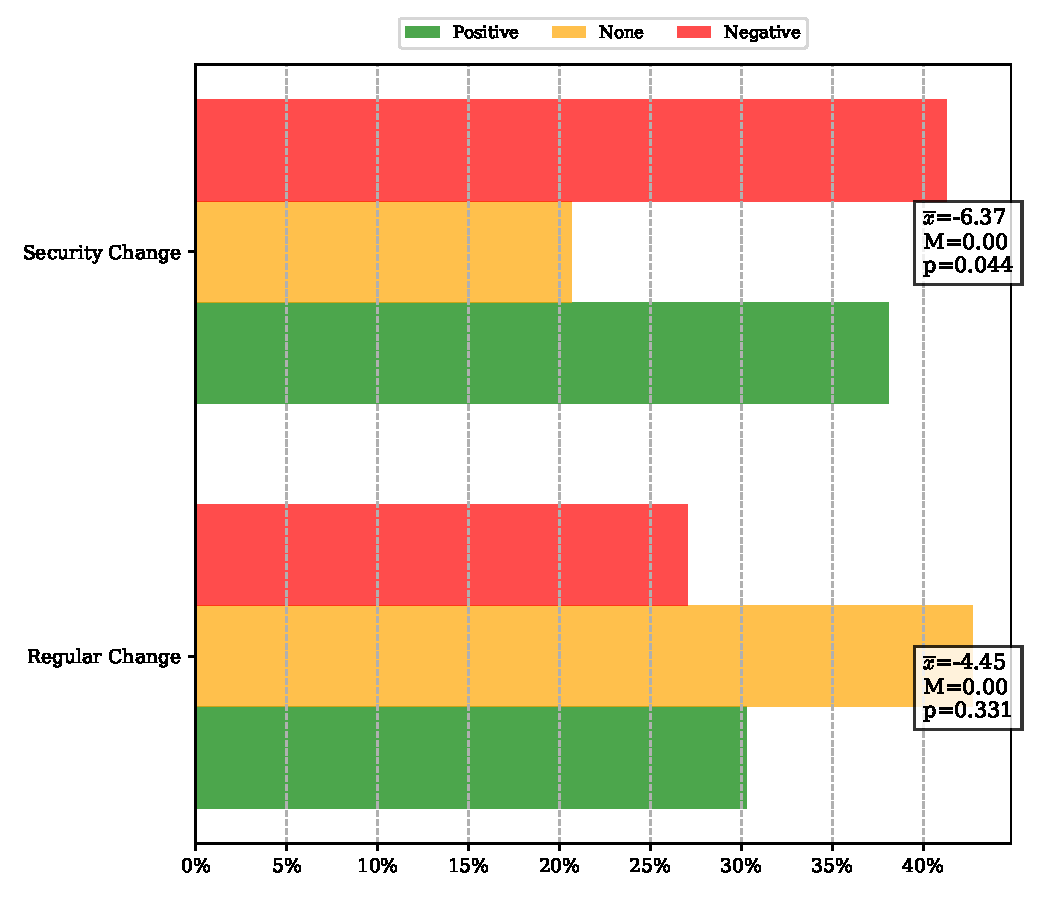
\includegraphics[width=0.7\textwidth]{figures/main_comparison.pdf}
 	\caption{Maintainability difference for security and baseline patches.}
	\label{fig:secvsreg}
\end{figure}

Results show that regular changes are less prone to hinder the software maintainability of open-source software.   
We manually inspected a considerable amount of cases from
the distribution of the regular changes where maintainability 
increases and found that identifying regular commits as similar in 
size as the security-related commit is limiting the type of regular 
commits being randomly chosen (e.g, input 
patches, variables or functions, type conversion, etc).  
We presume that this phenomenon lead
to the significant number of cases where there is no impact
on the software maintainability.

\textbf{Summary:} Security-related commits are observed to harm software 
maintainability. In contrast, one cannot say the same about
regular changes, in which \textbf{no significant differences are observed}. 
Thus, we urge the importance of adopting maintainability practices while 
applying security patches.

%
% For both types of changes, there is a negative impact
% on software maintainability---especially, for security changes.
% The resulting p-value of the Paired Wilcoxon signed-rank test is $0.300$, i.e.,
% conclusions regarding the regular changes are not statistically significant.
% Yet, it is important to note that \emph{patching security vulnerabilities seem
% to have a more negative impact on the maintainability of open-source software
% than performing regular changes}.
% This raises
% a new trade-off when developers need to patch vulnerabilities on their projects
% because they might be hindering the software maintainability or even introducing
% new vulnerabilities.


\section{Study Implications}\label{sec:implications}
%
Our results show evidence that developers may have to reduce maintainability for the 
sake of security. We argue that developers should be able to patch and produce 
secure code without hindering the maintainability of their projects. But there are 
still concerns that need to be addressed and that this study brings awareness for:
%

\textit{\textbf{Tools for Patch Risk Assessment:}}
	Design debt of one guideline can lead to severe impacts on the 
	software quality~\cite{10.1145/1985362.1985366}. Some software 
	producers consider security as a first class citizen while others 
	do not. As mentioned in previous work, security it is very important 
	and should bee considered as a default feature~\cite{10.1145/2489828.2489830,kurilova2014wyvern,mcgraw2004software}. 
	However, the lack of experts or awareness to the ease of producing 
	vulnerable software leads companies to ship low quality software. 
	Providing automated tools to developers assess the risk of their 
	patches it is important to help companies shipping software of higher quality. 
	Tools like Better Code Hub and static analysis (e.g., 
	SonarQube, Codacy, ESLint, Infer, and more) can be leveraged 
	to assess the risk of patching vulnerabilities---alongside pull
	requests/code reviews. Static code analysis may be daunting due 
	to the number of rules and different effects
	on maintainability. BCH claims to use the top-$10$ of the guidelines
	with the highest effects on maintainability. Yet, static analysis 
	can be used to complement the BCH analysis by introducing
	the capability of vulnerability detection and support the prediction 
	and prevention of the risk of a patch of hindering maintainability.
%

\textit{\textbf{Computer Science Curricula Needs to be Updated:}}
	Computer Science curricula is not yet prepared to properly educate 
	students for maintainable security. Students should be exposed to 
	this problem to gain experience with it. Curricula should focus on 
	the production of secure and maintainable code and alert to the 
	trade-off between both. These matters should be discussed and 
	presented to students in software engineering courses.
	Universities should also encourage students to use code quality 
	analysis tools such as BCH or similar ones. These tools have a 
	great potential to make students aware of maintainability issues 
	and beginner mistakes (e.g., coding practices violation).
%	

\textit{\textbf{More Secure Programming Languages Wanted:}} Programming 
	Languages should provide new design patterns to easily patch security weaknesses 
	without endangering maintainability. Ultimately, new programming languages, 
	both secure and maintainable by design, such as Wyvern~\cite{10.1145/2489828.2489830,kurilova2014wyvern}, 
	should be designed to help developers be less vulnerability prone when 
	writing and maintaining secure applications. One example is the need for 
	designing new authorization mechanisms since these are one of the most 
	complex security features to implement.
% 
% \\\textit{\textbf{Poor Coding Practices Documentation:}}
%   \Rui{too generic?}
% 	Software documentation must be provided to developers with the
% 	best practices to implement secure and maintainable software. Unmaintainable
% 	code is difficult to test, analyze and re-use. Software companies must
% 	do an effort to provide these artifacts to their developers, in order,
% 	to avoid the introduction of new vulnerabilities while patching older ones.

\section{Threats to Validity}\label{sec:threats}
%
This section presents the potential threats to validity of this study.
%

\textit{\textbf{Construct Validity:}} The formula to calculate the maintainability value ($M(v)$) was inferred based 
on the BCH's reports. The high amount of different projects and backgrounds 
may require other maintainability standards. However, BCH does use a 
representative benchmark of closed and open-source software projects to compute 
the thresholds for each maintainability guideline~\cite{Visser:2016:OREILLY,baggen2012}.
Maintainability is computed as the mean of all guidelines. Different software versions 
(vulnerable/fixed) of one vulnerability may have the same overall score
and still be affected by different guidelines. Therefore, we provide
an analysis per guideline and our results are all available on figshare for future reproductions and deeper analysis. 

\textit{\textbf{Internal Validity:}} The security patches dataset provided by previous
work~\cite{Reis:2017:IJSSE} was collected based on the messages of GitHub
commits produced by project developers to classify the changes performed while 
patching vulnerabilities. This approach discards patches that were
not explicit in commits messages. We assume that patches were performed 
using a single-commit or several sequentially. The 
perspective that a 
developer may quickly perform a patch and later 
proceed to the refactor is not considered. We assume 
that all patches were only performed once. Depending 
on the impact of the vulnerability in the system, some 
vulnerabilities may have more urgency to be patched than 
others. For instance, a vulnerability performing a Denial-of-Service attack
which usually brings entire systems down may be more urgent to patch than a 
cross-site scripting vulnerability which usually does not have impact
on the systems execution but rather on the data accessibility.

Baseline commits are retrieved randomly from 
the same project of the security patch.
This approach softens the differences
that may result from the characteristics of each project. However,
maintainability may still be affected by the developers' experience, coding
style, and software contribution policies which are not evaluated in this study.
Furthermore, this evaluation considers that $969$ regular commits---any kind
of commit---are enough to
alleviate random irregularities in the maintainability differences of the
baseline. 
%

\textit{\textbf{External Validity:}} The BCH tool uses private and open-source data to determine the thresholds for each guideline. We only analyze patches of open-source software.
Thus, our findings may not extend to private/non-open source software. Different programming 
languages may require different coding practices to address software safety. The 
dataset comprises more commits in Java, i.e., the dataset may not be representative 
of the population regarding programming languages. For both datasets, we a manual validation of the message of the commits was performed. Only commits in English were considered. Thus, our approach does not consider 
patches in any other language but English.

\section{Related Work}\label{sec:rw}

Many studies have investigated the relationship between patches and
software quality. Previous work focused on object-oriented metrics has evaluated the
impact of patches and exhibited proof that quantifying effectively the
impact of patches on maintainability may help to choose the appropriate
patch type~\cite{1167822}. In contrast to this work, Hegedus et
al.~\cite{HEGEDUS2018313} did not select particular metrics to assess the effect
of patches. Instead, statistical tests were used to find the metrics that
have the potential to change significantly after patches. 

Researchers
performed a large-scale empirical study to understand the characteristics of security patches
and their differences against security bug fixes~\cite{10.1145/3133956.3134072}.
The main findings were that security patches are smaller and less complex compared
to bug fixes and usually performed at function-level.

Studying the evolution 
of maintainability issues during the development of Android apps, Malavolta et al. ($2018$)~\cite{8530041}
discovered that maintainability decreases over time. Palomba et al.
($2018$)~\cite{Palomba:2018:DIM:3231288.3231337} exhibits proof that code smells
should be carefully monitored by programmers since there is a high correlation
between maintainability aspects and proneness to changes/faults. In 2019, Cruz et 
al.~\cite{8919169} proposed a formula to calculate maintainability 
based on the BCH's guidelines and measured the impact of energy-oriented fixes 
on software maintainability. Recent work,
proposed a new maintainability model to 
measure fine-grained code changes by adapting/extending the BCH model~\cite{8785997}.
The present work uses the same model (SIG-MM), considers more guidelines and focuses 
solely on evaluating the impact of security patches on software maintainability.

Researchers investigated the relationship between design patterns and
maintainability~\cite{10.1007/978-3-642-35267-6-18}. However, other studies show that 
the use of design patterns may introduce maintainability issues into
software~\cite{4493325}. Yskout et. al did not detect if the usage of 
design patterns has a positive impact but concluded that developers prefer to 
work with the support of security patterns~\cite{8077802}. The present work 
studies how security weaknesses influence maintainability for open-source software.

There are studies that investigated the impact of programming languages on software
quality~\cite{Ray:2014:LSS:2635868.2635922,Ray:2017:LSP:3144574.3126905}. The first
one shows that some programming languages are more buggy-prone than others. However,
the authors of the second one were not able to reproduce it and did not obtain any
evidence about the language design impact. 
Berger et al. ($2019$)~\cite{2019arXiv190110220B} tried to reproduce~\cite{Ray:2014:LSS:2635868.2635922,Ray:2017:LSP:3144574.3126905} 
and identified flaws that throw into distrust the 
previously demonstrated a correlation between programming language and software 
defects. Our work studies how security patches affect software quality based 
on the code maintainability analysis and provides shows that programming languages 
may have an impact on maintainability.

\section{Conclusion and Future Work}\label{sec:conclusions}

This work presents an empirical study on the impact of $969$ security
patches on the maintainability of $260$ open-source projects. We leveraged
Better Code Hub reports to calculate maintainability based on a model proposed in 
previous work~\cite{Olivari:2018,8919169}. Results show evidence of a 
trade-off between security and maintainability, as $41.9\%$ of security patches 
yielded a negative impact. Hence,
developers may be hindering software maintainability while patching 
vulnerabilities. We also observe that some guidelines 
and programming languages are more likely to be affected than others. The implications 
of our study are that changes to codebases while patching 
vulnerabilities need to be performed with extra care; tools
for patch risk assessment should be integrate into the CI/CD pipeline; computer science
curricula needs to be updated; and, more secure programming languages are necessary.

As future work, the study extended in several directions: 
investigate which guidelines affect most the maintainability per
weakness; check if vulnerability patches are followed by patch
commits and how much time does it take to do it; 
expand our methodology with other software quality properties; 
validate these findings with closed/private
software; and, expand this analysis to other quality standards.

% \section{Plan A}
%
% Please, pay more attention to the cases with !.
%
% \begin{itemize}
	% \item How this is a problem or has an impact to the software project?
	%   What is the message to developers? (clarify)
	% \item Implications: Discuss that depending on the project, maybe security
	%   is a first class citizen and should be fixed above all. Don't
	%   just state that patch risk assessment should take maintainability into account.
	%   Saying that security should be a priority requires maybe a user study
	%   as evidence (check if the literature available is not enough).
	%   \item Implications: Review the secure programming languages implication. Check
	%   if the idea of fully secure exists. The idea should be more secure, not
	%   fully secure.
  % \item [!] Implications: \textit{I am not sure how the computer science curricula got mentioned
  %   from a motivation. I don't think vulnerabilities are been introduced, its
  %   more that they get exposed. In this case, the implication does not make
  %   much sense from a practical point of view.} -> Why not? Shouldn't
  %   maintainable security be introduced in the computer science curricula since
  %   we have evidence that developers might not following good practices while
  %   patching? If they learn it in college and are aware of it in their jobs
  %   won't they be better prepared?
  % \item [!] \textit{It did take me several readings to understand the paper, especially the approach} -
 %  what to do with this @rui?
 %    \begin{itemize}
 %      \item Ehmm... strange... we need to improve the approach then. Thoughts?
 %    \end{itemize}
  % \item [!] \textit{Fig 4, although it looks impressive, I am not sure how to read the figure} - what
  % should we do @rui?
  %   \begin{itemize}
  %     \item Carefully explain it in the caption?
  %   \end{itemize}
  % \item [!] \textit{Fig 5, 6 and 7 are not the best ways to portray your findings. For instance, I am
  % still not sure how the positive, none and negative metrics are calculated and normalized} - what
  % is the best way then?
  %   \begin{itemize}
  %     \item Strange comment...
  %   \end{itemize}
  % \item \textit{Authors carefully highlight the key messages of each research question and answer
  % all accordingly} - Improve this.
  % \item [!] T2v: \textit{wrong assumption: patching commit should also be responsible to preserve the
  % maintainability.... The patching commit is to fix the vulnerability and to put the system is
  % an error-free, executable state so that the fix can be tested} -> I agree with this for vulnerabilities
  % that are the result of errors. For example, a bad expection handling, a memory leak that led to
  % a denial-of-service attack, NPE, etc. However, there are many other vulnerabilities whose
  % exploits do not have interference on systems execution. So, what to do here? Should we divide
  % the study by vulnerabilities and their implications on systems? Should we divide it by severity levels?
  %   \begin{itemize}
  %     \item We need to discuss this... I think this related to the next point.
  %   \end{itemize}
  % \item \textit{authors write "...important to write maintainable code to support the production
  % of more secure software...". Relationship is not clear nor is it backed by some evidence} ->
  % Improve this.
  % \item Drop the word patch. Security patches are not patches. Refactorings is perfective
  % or preventive maintenance, whereas patching a vulnerability is corrective maintenance.
  % \item Discuss better the fact of not using other important aspects for the baseline such as the
  % size of the changed method and complexity by metrics. Soften the part where it says we should
  % have gone beyond size.
  % \item \textit{ Figure 4 does not indicate that or support the statement that “patching
  % vulnerabilities has a very significant number of negative cases for all guidelines”. Besides a
  % corresponding statistical test that supports this statement, even the swarm and box plotz itself
  % clearly tell a different story. So, authors may rethink this statement or better explain how they
  % come to this conclusion.} -> We are overselling here. Improve it.
  % \item \textit{Authors state that they assume for the Pontas dataset that the last commit related
  % to patching being the actual patch while the parent of the first patch-related commit is assumed
  % to be the vulnerable version. However, nothing is said whether this assumption holds all the time.
  % So, how did authors validate their assumption? This is missing, but should be added.} - Improve this.
  % \item \textit{In Section 3-C, for computing and comparing the maintainability, only security commits
  % (and parent commit) are mentioned. Did you apply the same method also the the regular changes that
  % you use to compare with security commits? Please make this clear, currently this is ignored in the
  % particular  (sub) section.} - Improve this.
  % \item \textit{For clarification, the authors explained that they performed a manual investigation
  % for RQ3. It would be beneficial for more details.} -> Clarify this.
  % \item \textit{In terms of presentation, the results were a bit difficult to follow at times as they
  % did not contain contextualization. For example, “negative cases” can seem a bit ambiguous when
  % referencing the relationship between the impact with guidelines.} -> Improve this.

% \end{itemize}

% \section{Plan B}
%
% Baseado nos reviewers, eu acho que para seguir as orientaçoes deles de refletir e fortalecer
% a nova assumption e as implicaçoes, teriamos de acrescentar ao Plano A, os proximos pontos
% antes de submeter à ESME.
%
% \begin{itemize}
% \item \textbf{Step 1:} Pegar nos casos em que o impacto na maintainability foi negativa e ver se foram modificados
% depois e se sim, se houve melhoria da maintainability. -> isto para então resolver a questao da
% assumption errada.
% \item \textbf{Step 2:} Se não existir nenhuma alteração, entao talvez entrar em contacto com os developers
% e perguntar se quando fizeram o patch tiveram em consideração maintainability do projecto. E se não porquê.
% \item Problemas de baselines e testes acho que nao vale a pena pegar porque vai depender
% do reviewer (eu acho).
% \end{itemize}
%
% Qual é o plano que acha melhor? Como prosseguir?
%
% A discutir, mas acho que por agora era tentar fazer o 1.
%
% \section{Later}
%
% \begin{itemize}
% 	\item \textbf{Assumptions:}\textit{authors measure the maintainability directly after the patch. inestad it should look
%   for multiple follow up commits and how maintainability evolves there, as it is likely that certain
%   issues are addresses AFTER the patching commit} -> I think we should see if later commits touch on
%   the patch and measure their maintainability again. Was a less maintainable fix pushed first and then
%   refactored, or does the code stay less maintainable?
%   \item \textbf{To back up implications:} \textit{In terms of the push for changes to curricula, I would agree that it is important
%   to always stress writing high quality code. However, the support by the study is not strong. Given a
%   majority of patches did not decrease maintainability, it shows that there is a reasonable focus on maintainability.
%   Similarly, it is important to understand the circumstances when it decreased. As previously mentioned, organizations
%   like would prioritize getting the system patched faster (especially in the case of a severe vulnerability) over
%   its maintainability.} -> Work with practioners to understand if they were taking into consideration maintainability?
%   \item \textbf{Baseline:}\textit{Authors just search for commits of a similar size. There are other important aspects
%   that are entirely neglected such as size of the changed method or how complex it it (by means of
%   metrics)} -> Improve baseline.
%   \item \textbf{Baseline:}\textit{Similarly, the comparison to “regular” commits really compares security patches to
%   any other type of change. It would have been more meaningful to compared them to specific types of
%   commits, like bug fixes (e.g., are security fixes less maintainable than bug fixes?).}
%   \item \textbf{Tests:}\textit{or the chosen statistical test, the hypothesis may be not well chosen as it just checks for
%   the same distribution of pairs of versions. However, this means if a similar number of pairs have
%   a negative and a positive impact, the hypothesis holds however, if this is not the case, the statistical
%   test does not state in which direction the hypothesis is rejected, that is, what eventually is the
%   alternative hypothesis. But this is necessary to get insights whether maintainability is hampered or not.
%   Authors may rethink the choice of the hypothesis or even the test itself.} -> What about this?
%   \item \textbf{Thesis idea (PL):} It is important
%   to understand the correlation between the severity of the vulnerability and the programming language as well
%   as the maintainability impact. It is not clear how software written a more security-focused language would
%   inherently be more maintainable (it assumes the flaw is the language and not the person).
% \end{itemize}
 
\bibliographystyle{spmpsci}
\bibliography{emse20}   % name your BibTeX data base

\end{document}
% end of file template.tex

